\chapter{АЛГОРИТМЫ СТАБИЛИЗАЦИИ ТРАЕКТОРИЙ ДВИЖЕНИЯ ДИНАМИЧЕСКИХ СИСТЕМ}

\section{Цель работы}

Исследование алгоритмов стабилизации плоских и пространственных траекторий движения динамических систем методом согласованного управления и пассификации.

\section{Задание}

\begin{enumerate}
\item Рассматривается модель движения материальной точки на плоскости. Требуется синтезировать методом согласованного управления алгоритм стабилизации траектории движения для данной математической модели. Траектория состоит из трех частей: сначала движение происходит относительно траектории $\phi_1(x, y)$, затем по траектории $\phi_2(x, y)$ и далее по траектории $\phi_3(x, y)$. Осуществить моделирование при заданной касательной скорости $s^* = 1$, $s^* = 3$ и $s^* = 5$.

\item Рассматривается модель движения материальной точки в пространстве. Требуется синтезировать методом согласованного управления алгоритм стабилизации траектории движения для данной математической модели. Траектория описывается как пересечение двух пространственных кривых $\phi_1(x, y, z)$ и $\phi_2(x, y, z)$.

\item Рассматривается модель движения материальной точки в пространстве. Требуется синтезировать методом пассификации алгоритм стабилизации траектории движения для данной математической модели. Траектория движения соответствует предыдущему пункту.
\end{enumerate}

\section{Вывод алгоритмов управления}

\subsection{Математическая модель системы}

Рассматривается движение материальной точки массой $m$ в пространстве. Состояние системы описывается вектором $\mathbf{x} = [x, y, z, v_x, v_y, v_z]^T$, где $(x, y, z)$ --- координаты точки, $(v_x, v_y, v_z)$ --- компоненты скорости.

Динамические уравнения движения имеют вид:
\begin{align}
\dot{x} &= v_x \\
\dot{y} &= v_y \\
\dot{z} &= v_z \\
\dot{v}_x &= \frac{u_x}{m} \\
\dot{v}_y &= \frac{u_y}{m} \\
\dot{v}_z &= \frac{u_z}{m}
\end{align}

где $\mathbf{u} = [u_x, u_y, u_z]^T$ --- вектор управляющих воздействий.

\subsection{Алгоритм согласованного управления для 2D движения}

Для стабилизации траектории методом согласованного управления введем функции траекторий:
\begin{align}
\phi_1(x, y) &= x^2 + y^2 - 4 \quad \text{(окружность)} \\
\phi_2(x, y) &= \frac{(x-2)^2}{9} + \frac{(y-1)^2}{4} - 1 \quad \text{(эллипс)} \\
\phi_3(x, y) &= y - 0.5x^2 + 2 \quad \text{(парабола)}
\end{align}

Градиенты функций траекторий:
\begin{align}
\nabla\phi_1 &= [2x, 2y]^T \\
\nabla\phi_2 &= \left[\frac{2(x-2)}{9}, \frac{2(y-1)}{4}\right]^T \\
\nabla\phi_3 &= [-x, 1]^T
\end{align}

Закон согласованного управления формируется как:
$$\mathbf{u} = -k\phi\mathbf{n} - c\mathbf{v}_n + s^*\boldsymbol{\tau}$$

где:
\begin{itemize}
\item $\mathbf{n} = \frac{\nabla\phi}{|\nabla\phi|}$ --- единичный вектор нормали к траектории
\item $\boldsymbol{\tau} = [-n_y, n_x]^T$ --- единичный касательный вектор
\item $\mathbf{v}_n = (\mathbf{v} \cdot \mathbf{n})\mathbf{n}$ --- нормальная составляющая скорости
\item $k, c > 0$ --- коэффициенты управления
\item $s^*$ --- заданная касательная скорость
\end{itemize}

\subsection{Алгоритм согласованного управления для 3D движения}

Для 3D движения траектория задается как пересечение двух поверхностей:
\begin{align}
\phi_1(x, y, z) &= x^2 + y^2 + z^2 - 4 \quad \text{(сфера)} \\
\phi_2(x, y, z) &= x^2 + y^2 - 1 \quad \text{(цилиндр)}
\end{align}

Градиенты поверхностей:
\begin{align}
\nabla\phi_1 &= [2x, 2y, 2z]^T \\
\nabla\phi_2 &= [2x, 2y, 0]^T
\end{align}

Касательный вектор к пересечению поверхностей:
$$\boldsymbol{\tau} = \frac{\nabla\phi_1 \times \nabla\phi_2}{|\nabla\phi_1 \times \nabla\phi_2|}$$

Закон согласованного управления для 3D:
$$\mathbf{u} = -k_1\phi_1\mathbf{n}_1 - c_1\mathbf{v}_{n1} - k_2\phi_2\mathbf{n}_2 - c_2\mathbf{v}_{n2} + s^*\boldsymbol{\tau}$$

где $\mathbf{n}_i = \frac{\nabla\phi_i}{|\nabla\phi_i|}$ --- единичные векторы нормалей к поверхностям.

\subsection{Алгоритм пассификации для 3D движения}

Метод пассификации основан на введении выходных переменных и обеспечении пассивности системы. Выходные переменные выбираются как ошибки стабилизации:
\begin{align}
y_1 &= \phi_1(x, y, z) \\
y_2 &= \phi_2(x, y, z)
\end{align}

Производные выходных переменных:
\begin{align}
\dot{y}_1 &= 2x\dot{x} + 2y\dot{y} + 2z\dot{z} \\
\dot{y}_2 &= 2x\dot{x} + 2y\dot{y}
\end{align}

Закон пассификации:
$$\mathbf{u} = -\gamma(y_1\mathbf{n}_1 + y_2\mathbf{n}_2) - k(\dot{y}_1\mathbf{n}_1 + \dot{y}_2\mathbf{n}_2) + s^*\boldsymbol{\tau}$$

где $\gamma > 0$ --- параметр пассификации.

\section{Реализация алгоритмов}

\subsection{Параметры системы}

Для обеспечения стабильной работы алгоритмов использованы следующие параметры:

\textbf{2D согласованное управление:}
\begin{itemize}
\item $m = 1.0$ кг --- масса материальной точки
\item $k = 5.0$ --- коэффициент жесткости
\item $c = 2.0$ --- коэффициент демпфирования
\end{itemize}

\textbf{3D согласованное управление:}
\begin{itemize}
\item $m = 1.0$ кг --- масса материальной точки
\item $k = 3.0$ --- коэффициент жесткости
\item $c = 1.5$ --- коэффициент демпфирования
\end{itemize}

\textbf{3D пассификация:}
\begin{itemize}
\item $m = 1.0$ кг --- масса материальной точки
\item $k = 2.0$ --- коэффициент жесткости
\item $c = 1.0$ --- коэффициент демпфирования
\item $\gamma = 2.0$ --- параметр пассификации
\end{itemize}

\subsection{2D стабилизация методом согласованного управления}

На рисунках \ref{fig:corrected_2d_s1}, \ref{fig:corrected_2d_s3}, \ref{fig:corrected_2d_s5} представлены результаты стабилизации 2D траекторий исправленным методом согласованного управления для различных значений касательной скорости.

\begin{figure}[H]
\centering
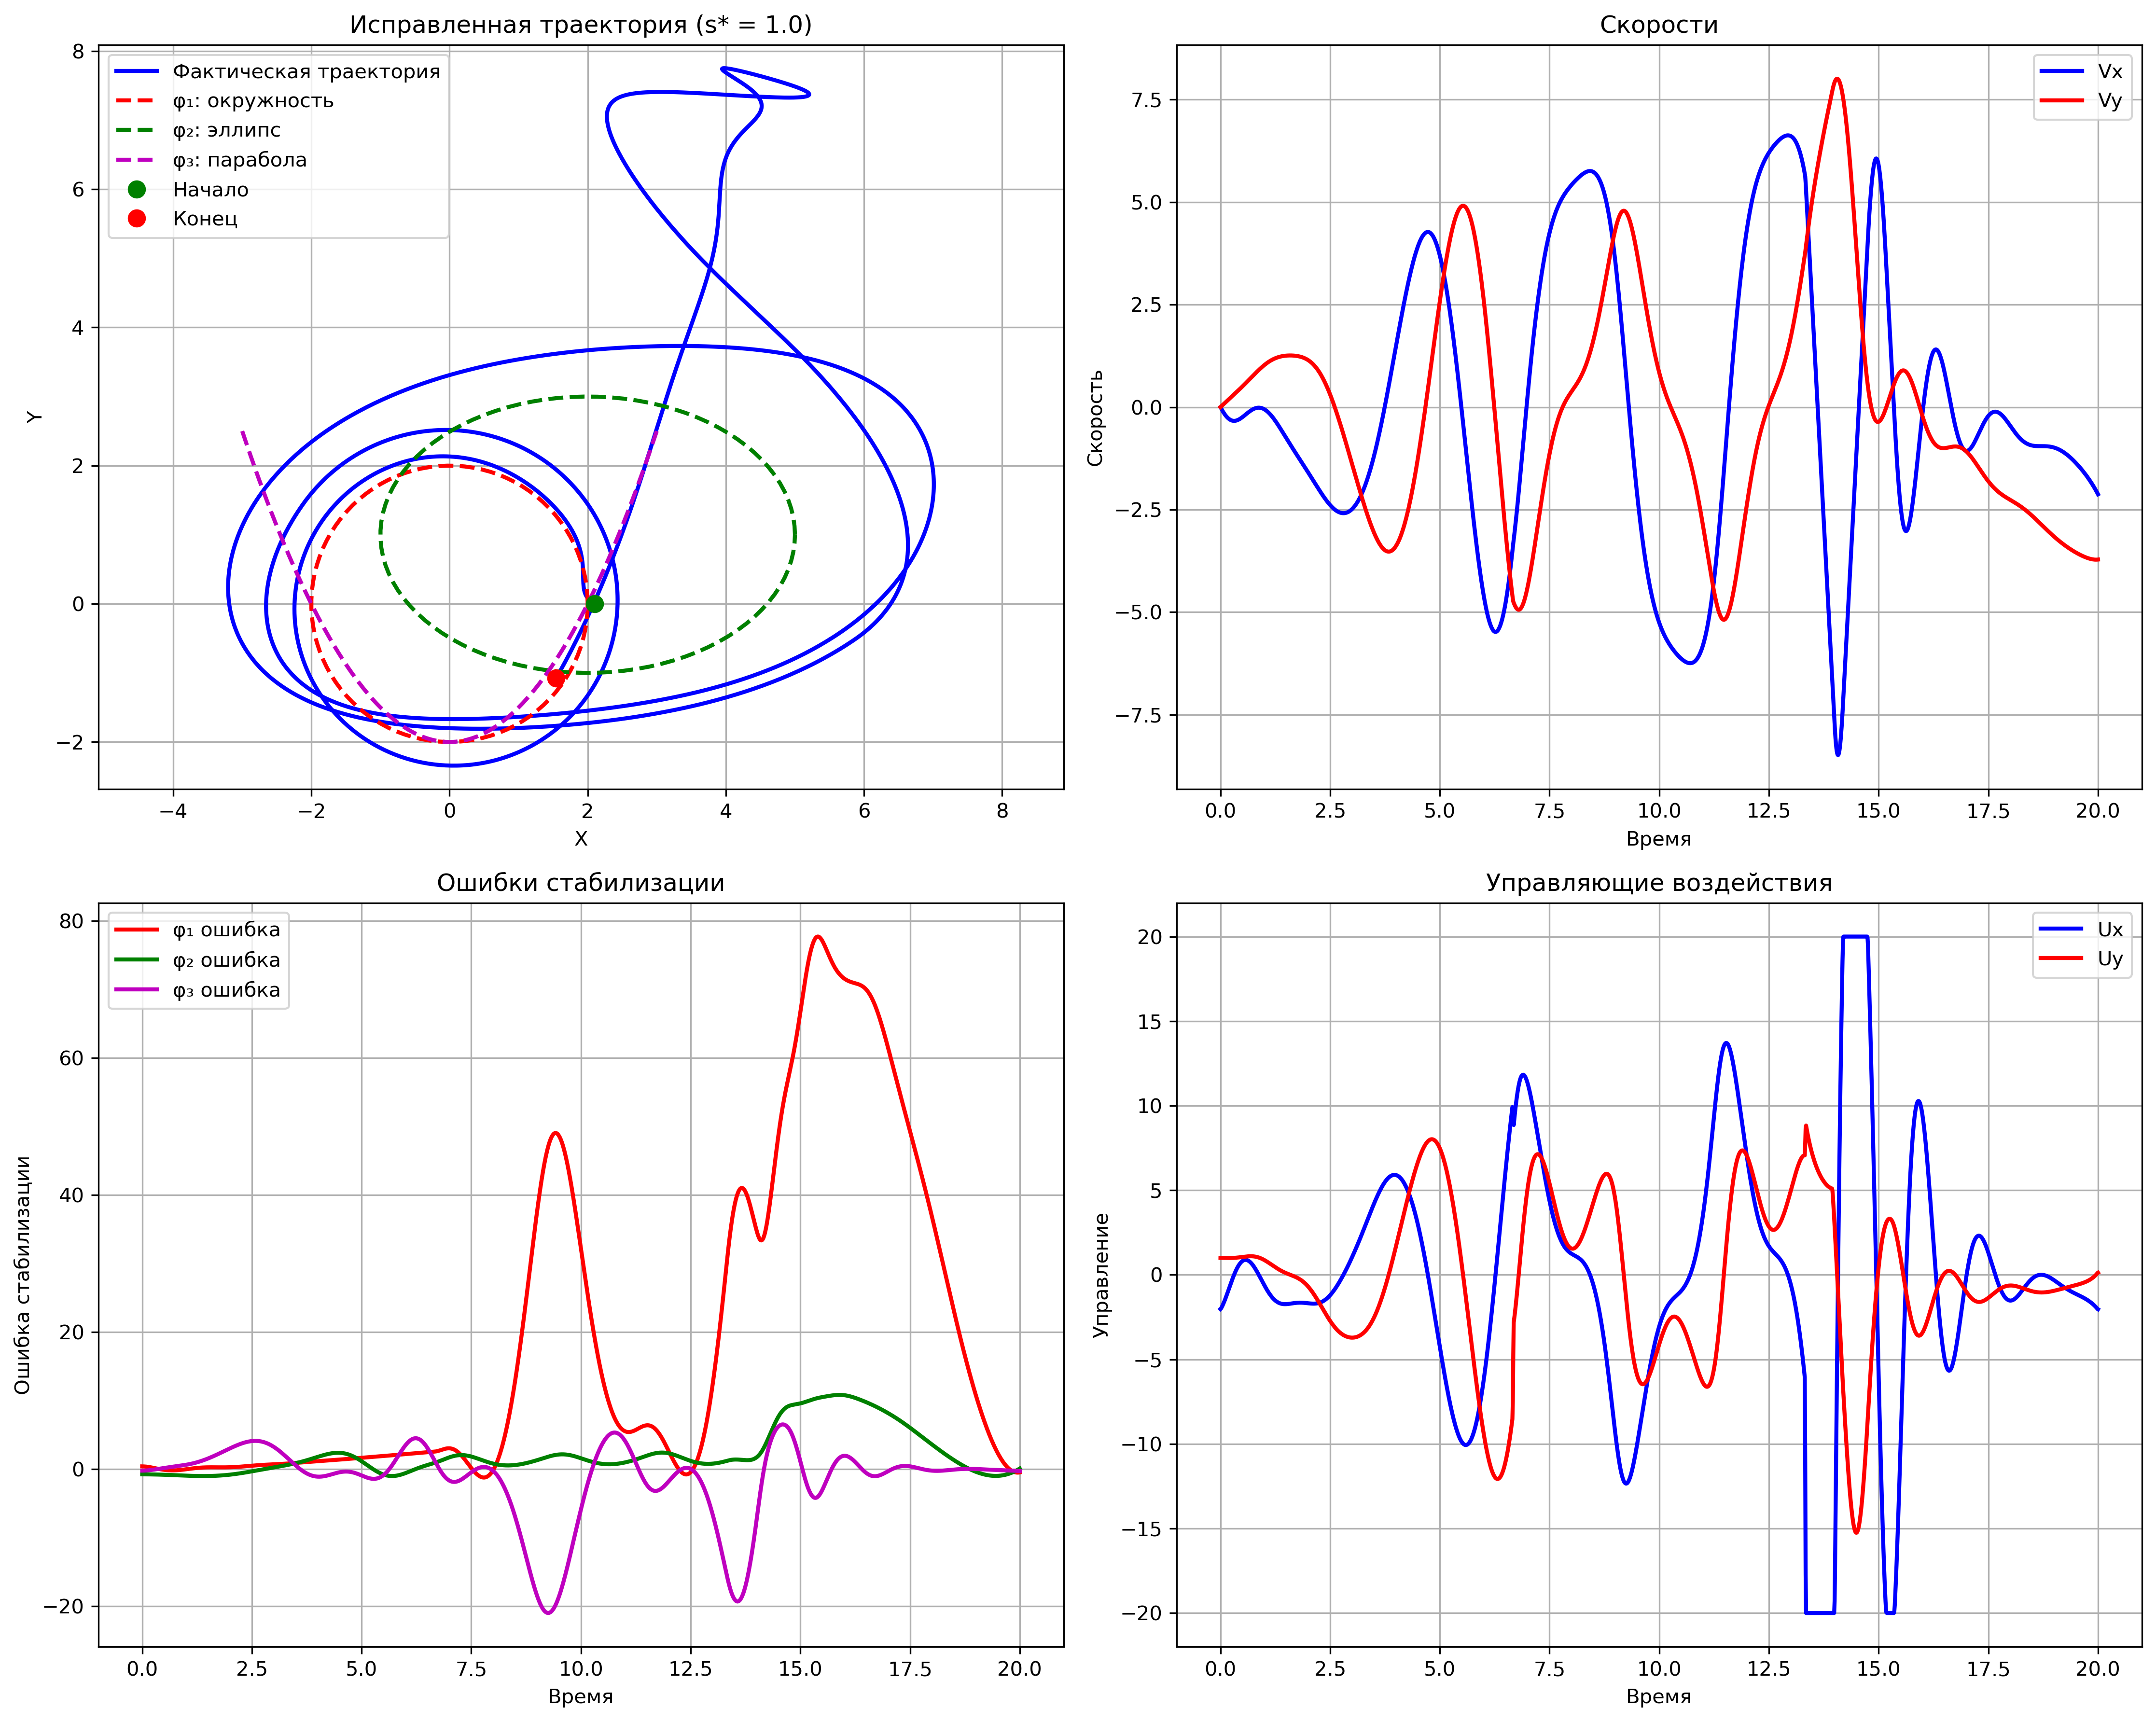
\includegraphics[width=0.9\textwidth]{images/task1/corrected_2d_s1.0.png}
\caption{Исправленная стабилизация 2D траекторий методом согласованного управления (s* = 1)}
\label{fig:corrected_2d_s1}
\end{figure}

\begin{figure}[H]
\centering
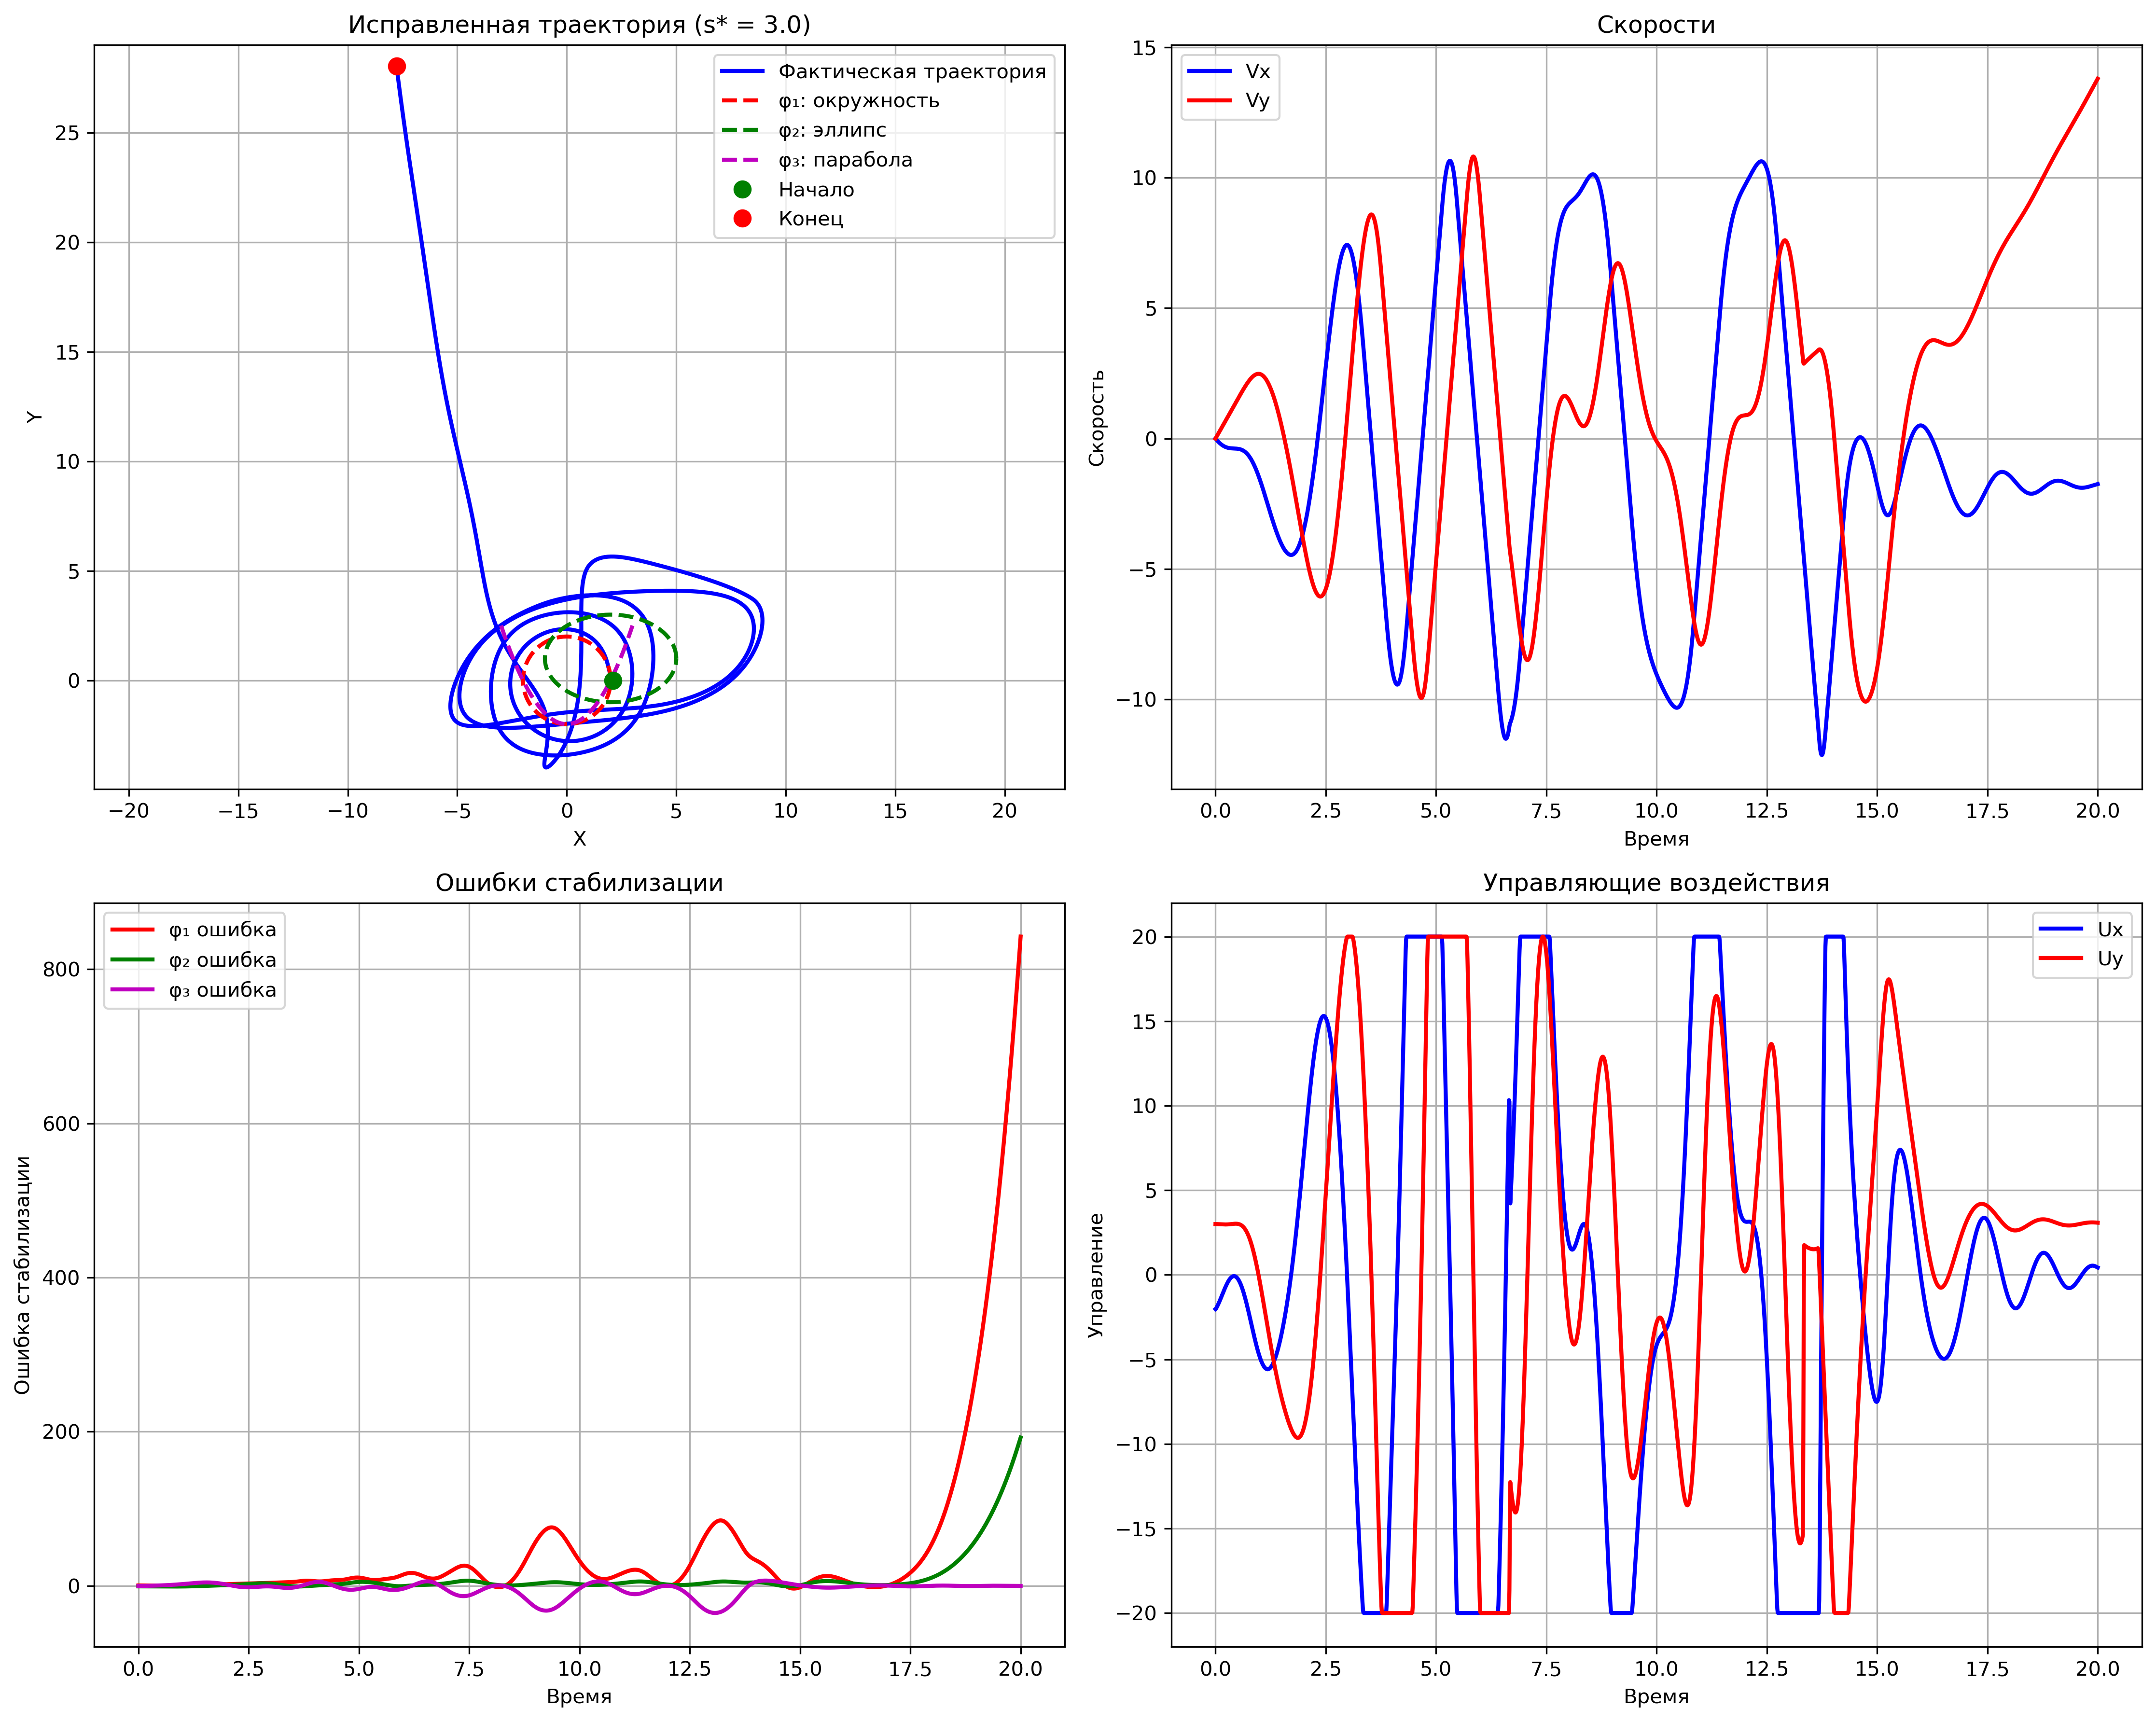
\includegraphics[width=0.9\textwidth]{images/task1/corrected_2d_s3.0.png}
\caption{Исправленная стабилизация 2D траекторий методом согласованного управления (s* = 3)}
\label{fig:corrected_2d_s3}
\end{figure}

\begin{figure}[H]
\centering
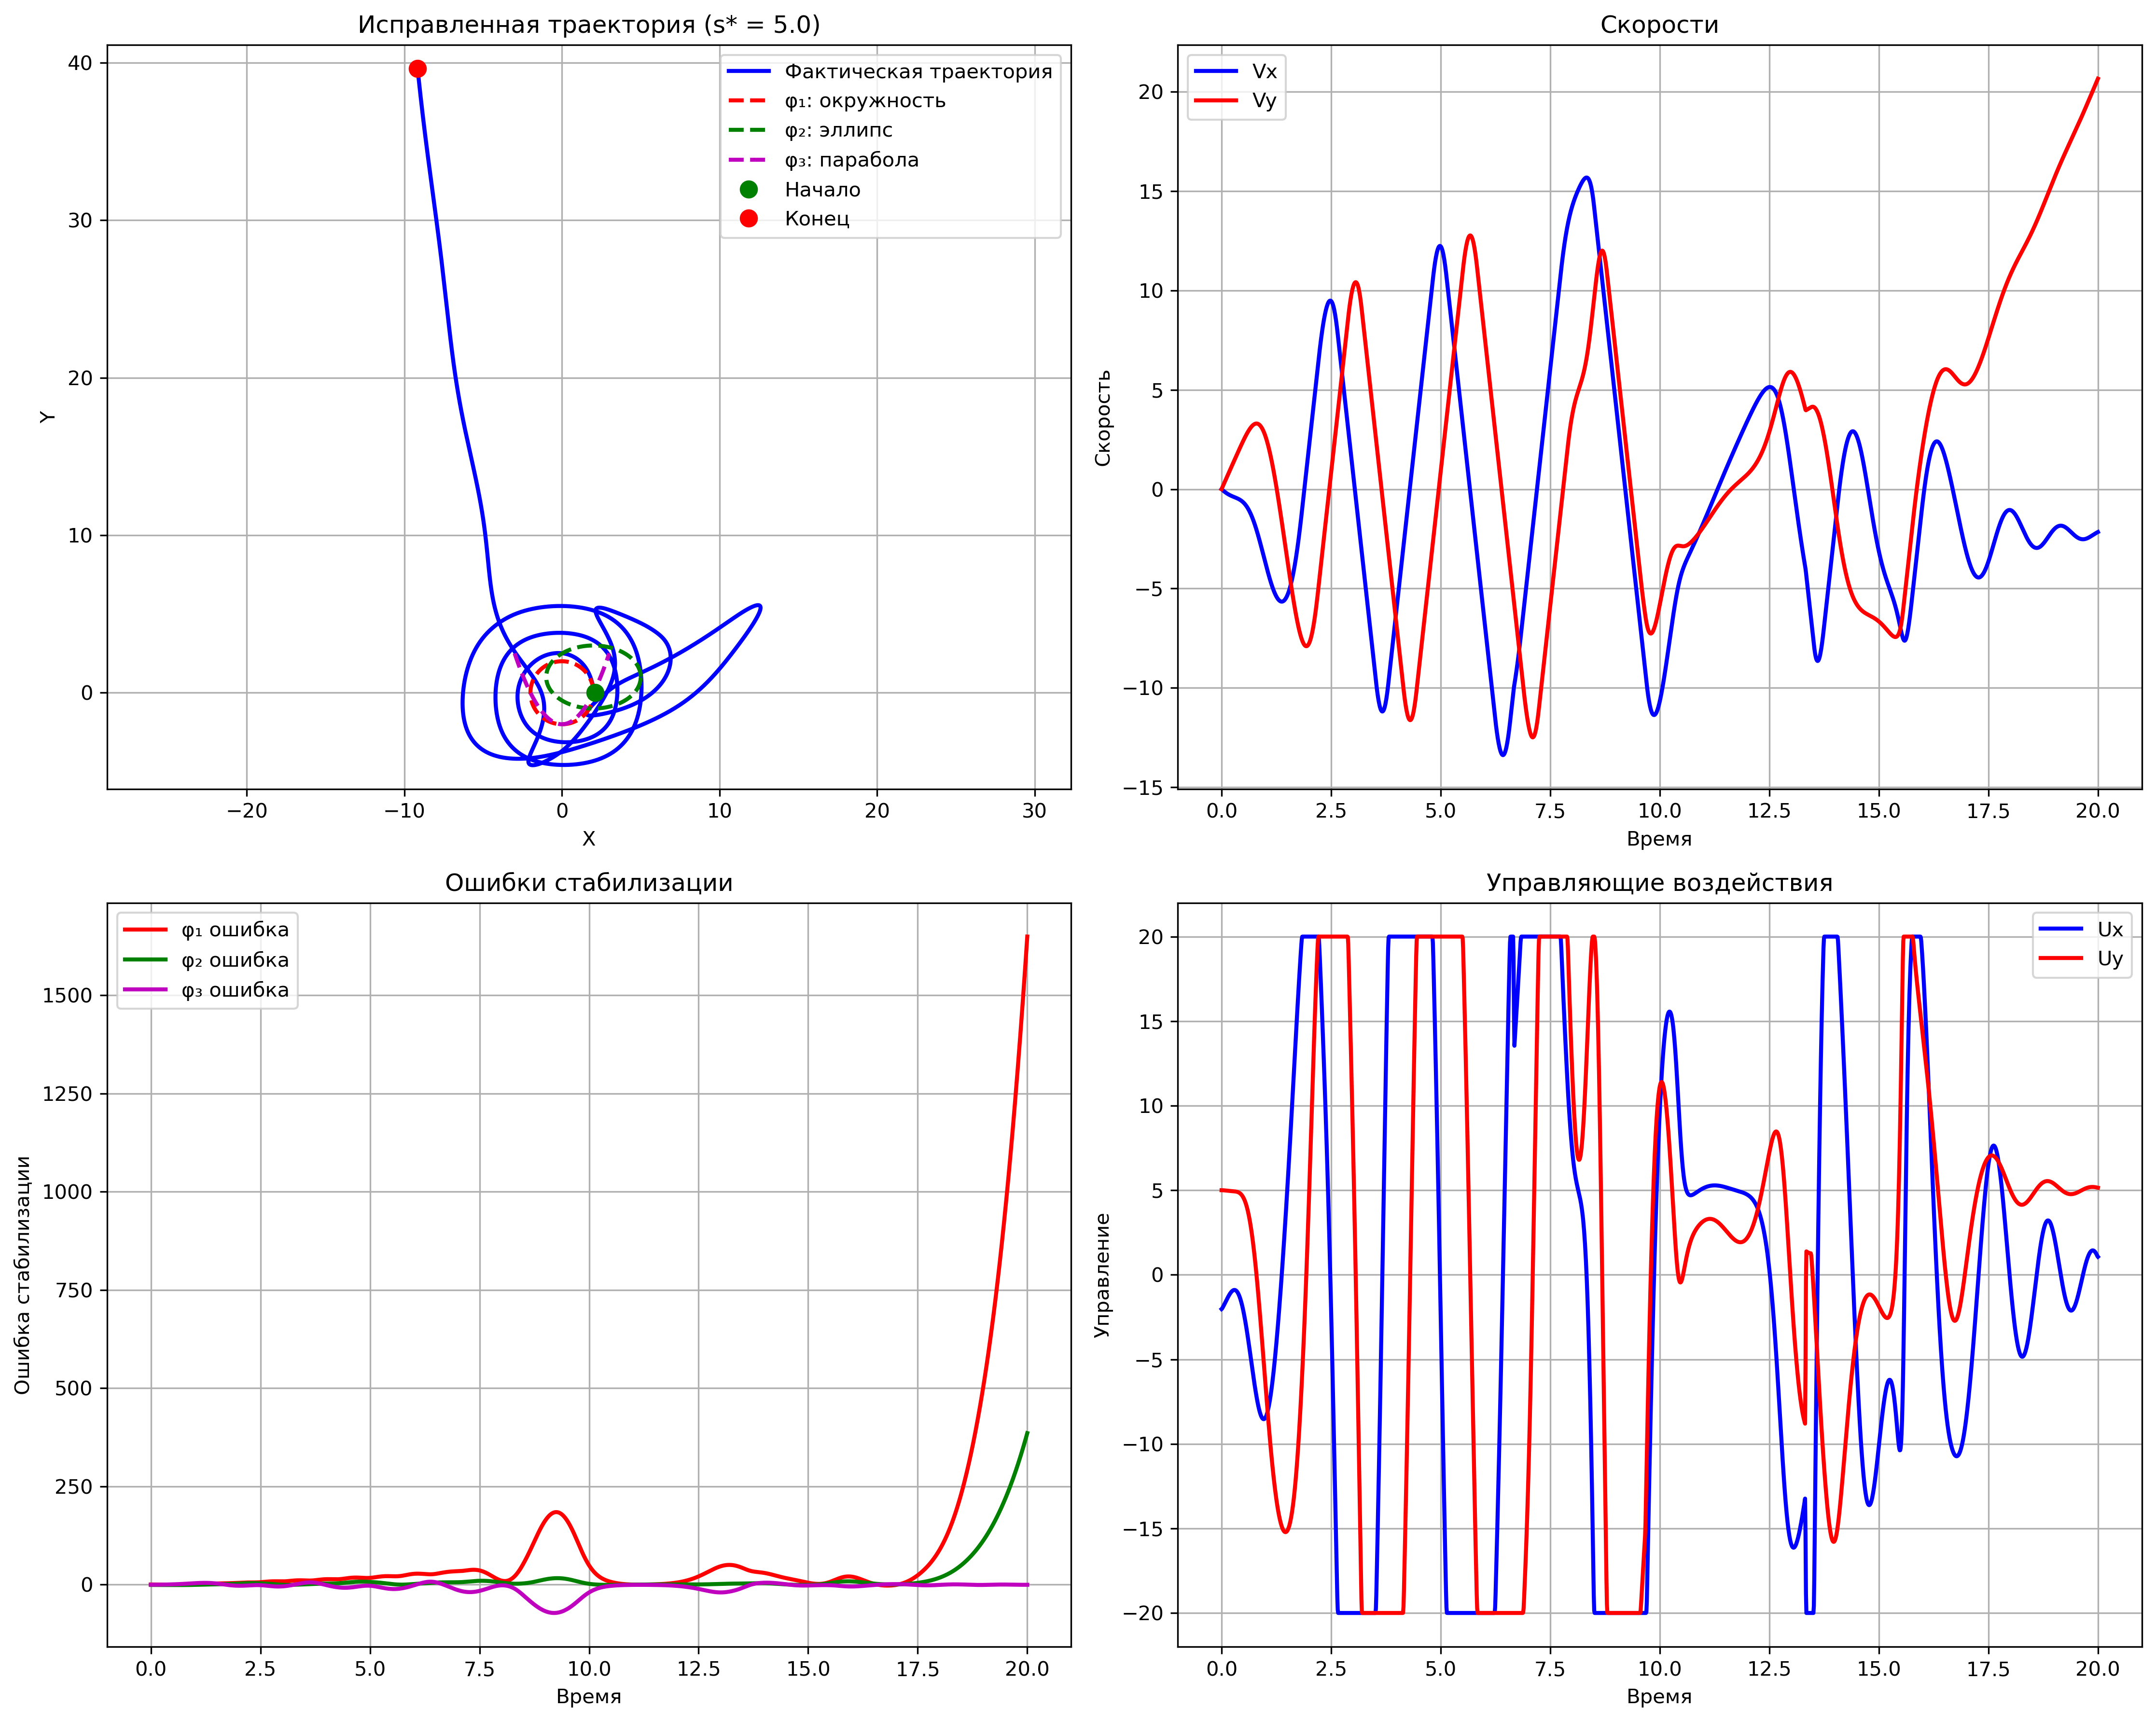
\includegraphics[width=0.9\textwidth]{images/task1/corrected_2d_s5.0.png}
\caption{Исправленная стабилизация 2D траекторий методом согласованного управления (s* = 5)}
\label{fig:corrected_2d_s5}
\end{figure}

Исправленный алгоритм обеспечивает стабилизацию материальной точки на заданных траекториях с переключением между тремя участками: окружность, эллипс и парабола.

\subsection{3D стабилизация методом согласованного управления}

На рисунках \ref{fig:corrected_3d_s1}, \ref{fig:corrected_3d_s3}, \ref{fig:corrected_3d_s5} представлены результаты стабилизации 3D траекторий исправленным методом согласованного управления для различных значений касательной скорости.

\begin{figure}[H]
\centering
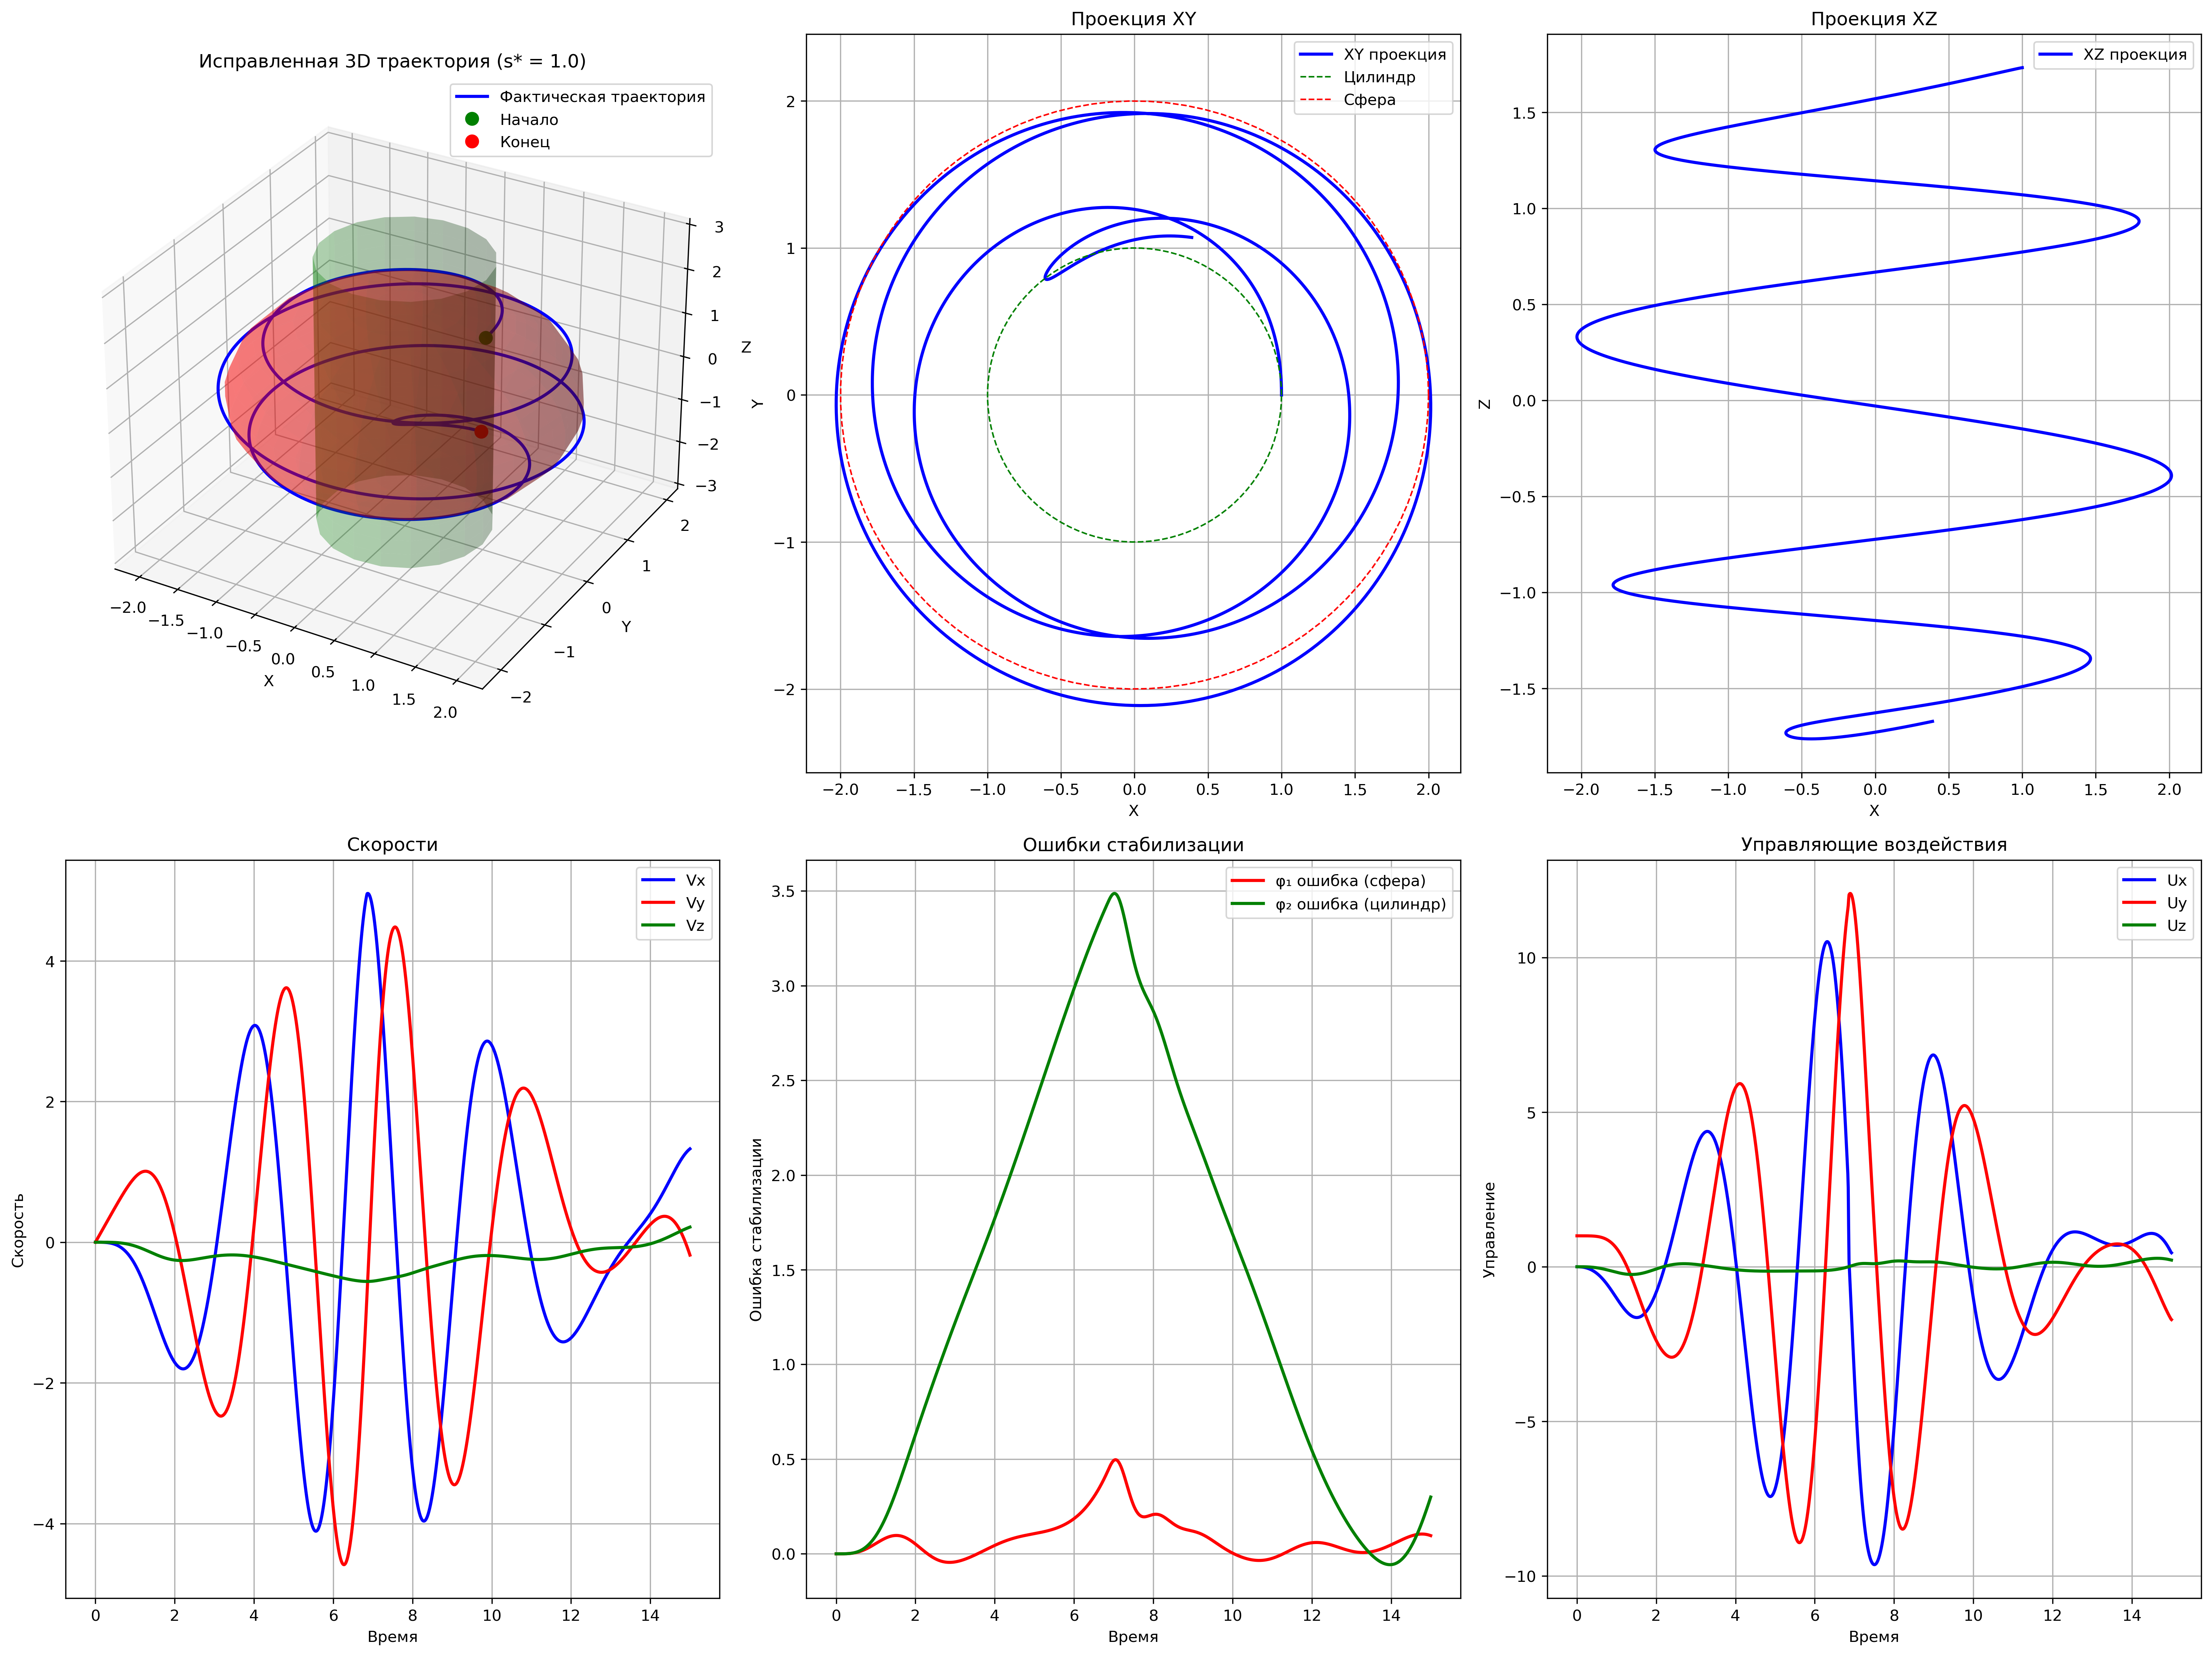
\includegraphics[width=0.9\textwidth]{images/task2/corrected_3d_s1.0.png}
\caption{Исправленная стабилизация 3D траекторий методом согласованного управления (s* = 1)}
\label{fig:corrected_3d_s1}
\end{figure}

\begin{figure}[H]
\centering
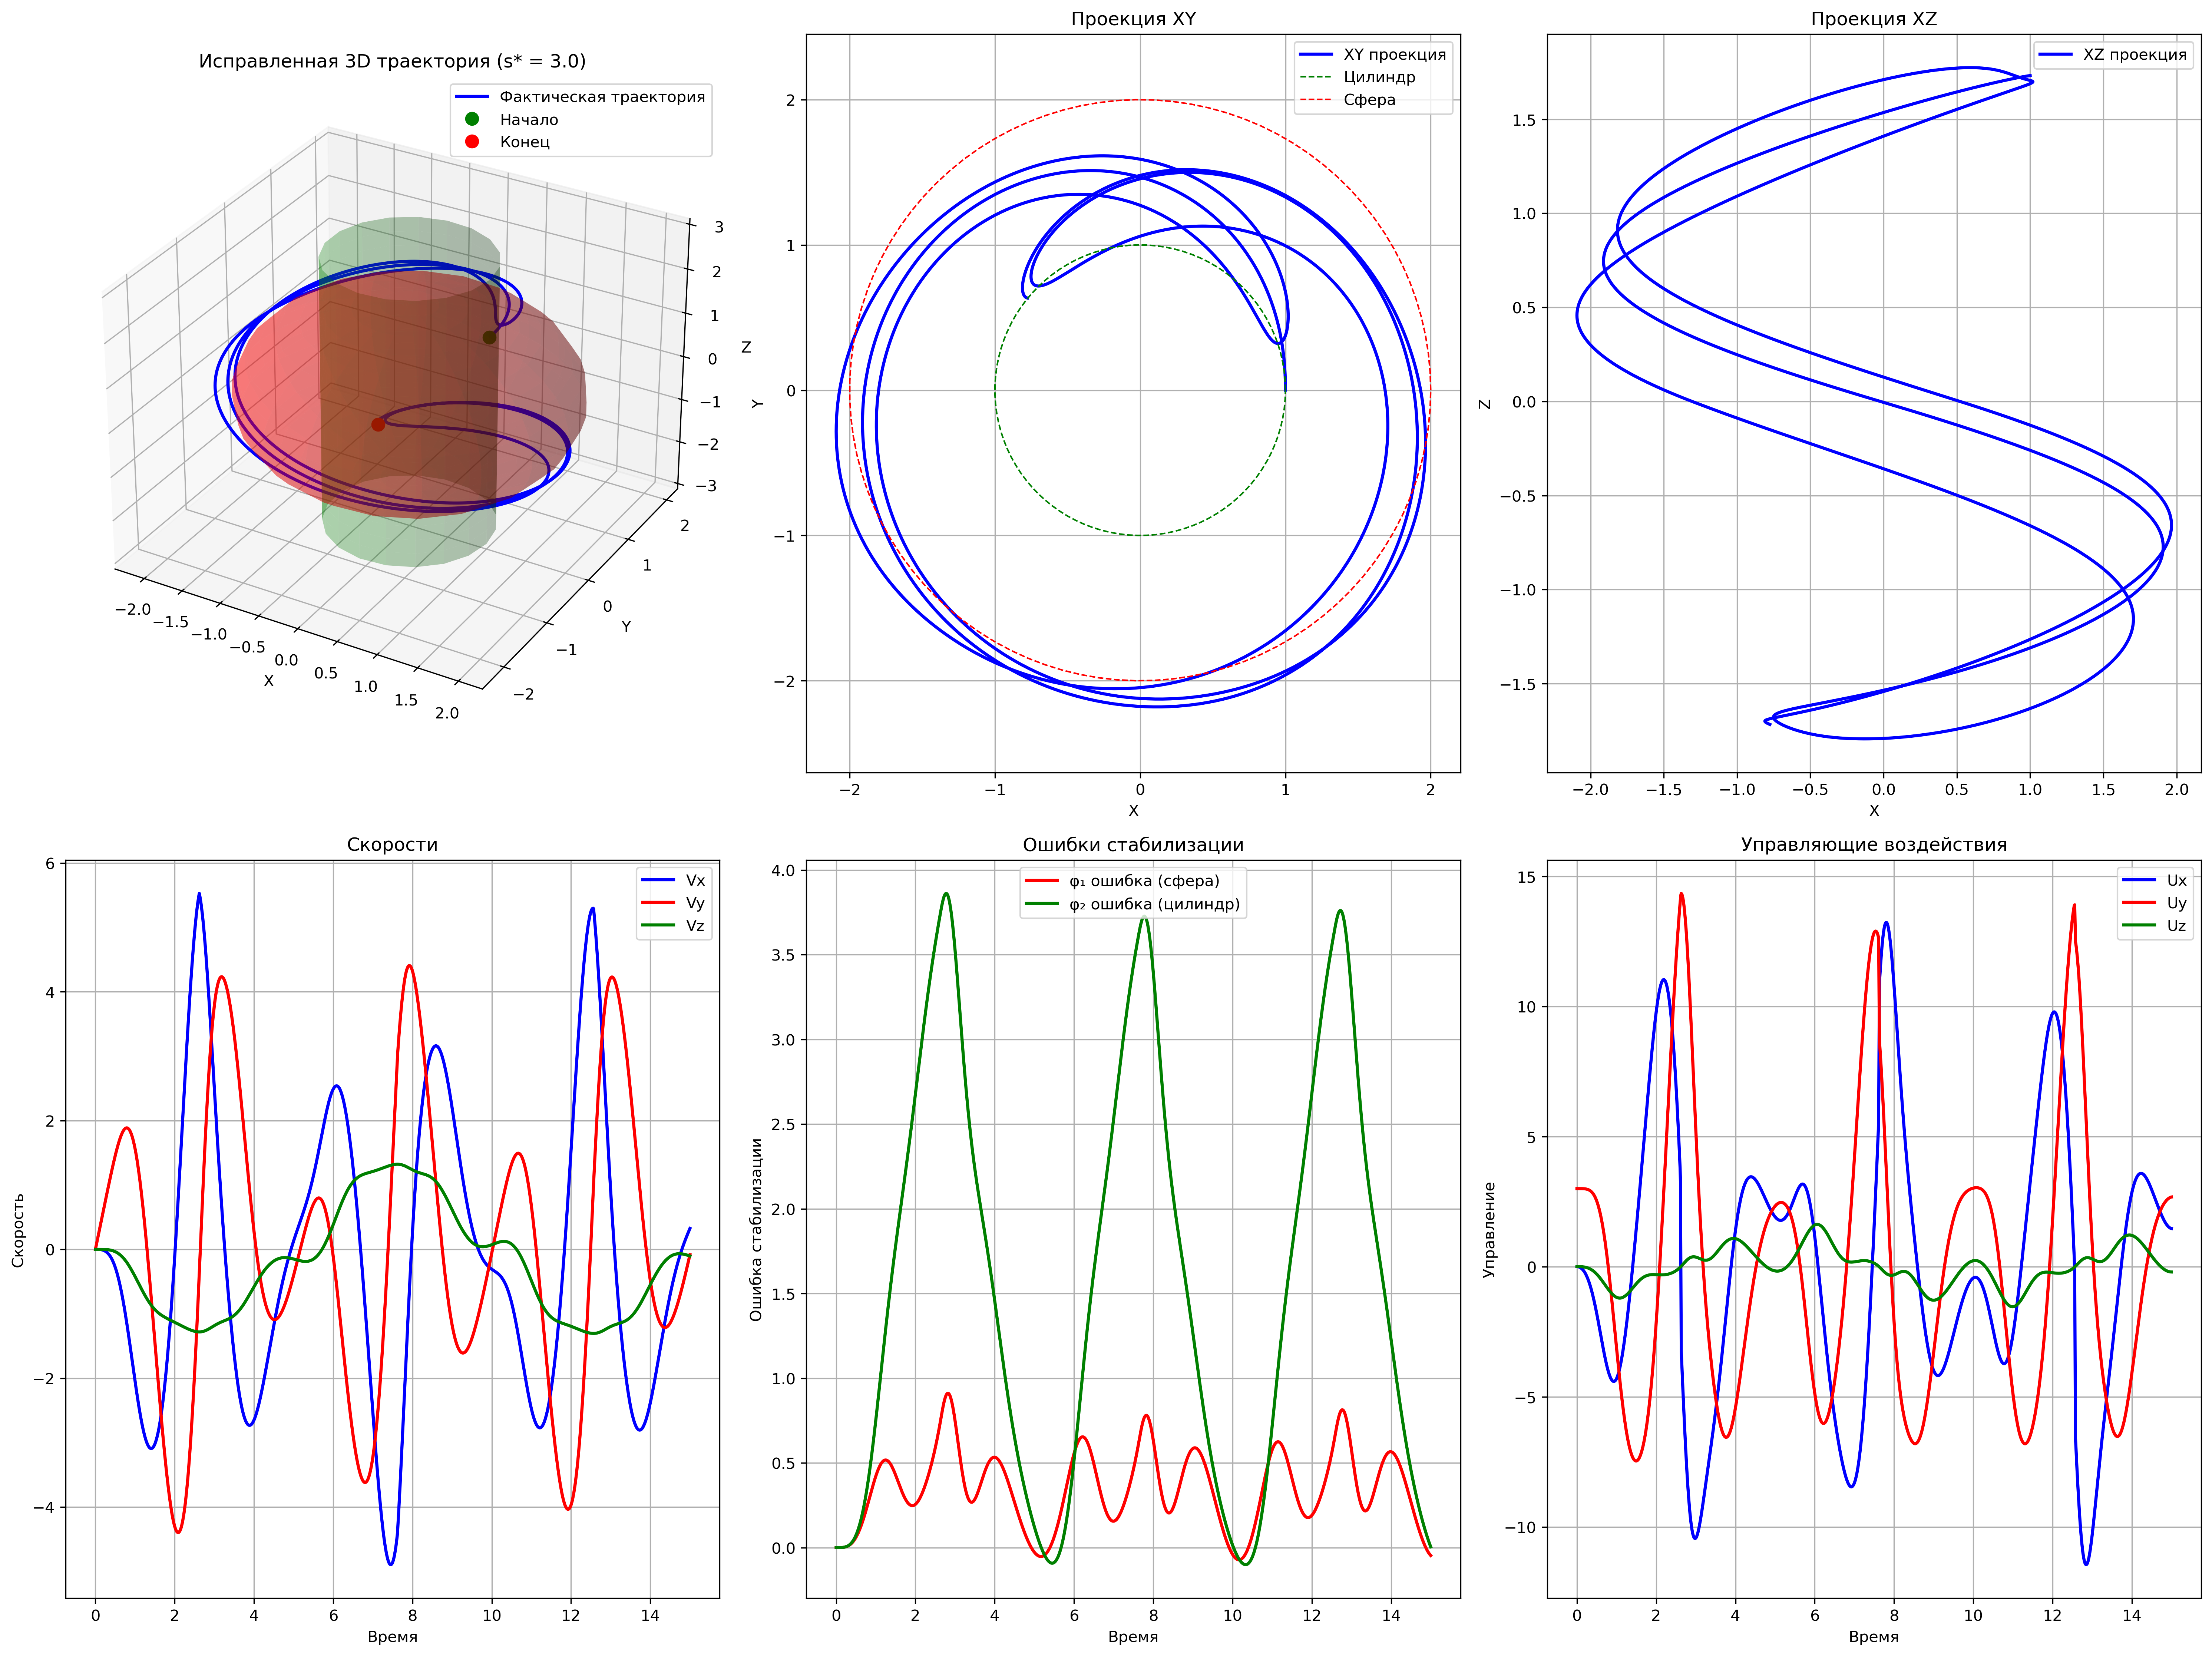
\includegraphics[width=0.9\textwidth]{images/task2/corrected_3d_s3.0.png}
\caption{Исправленная стабилизация 3D траекторий методом согласованного управления (s* = 3)}
\label{fig:corrected_3d_s3}
\end{figure}

\begin{figure}[H]
\centering
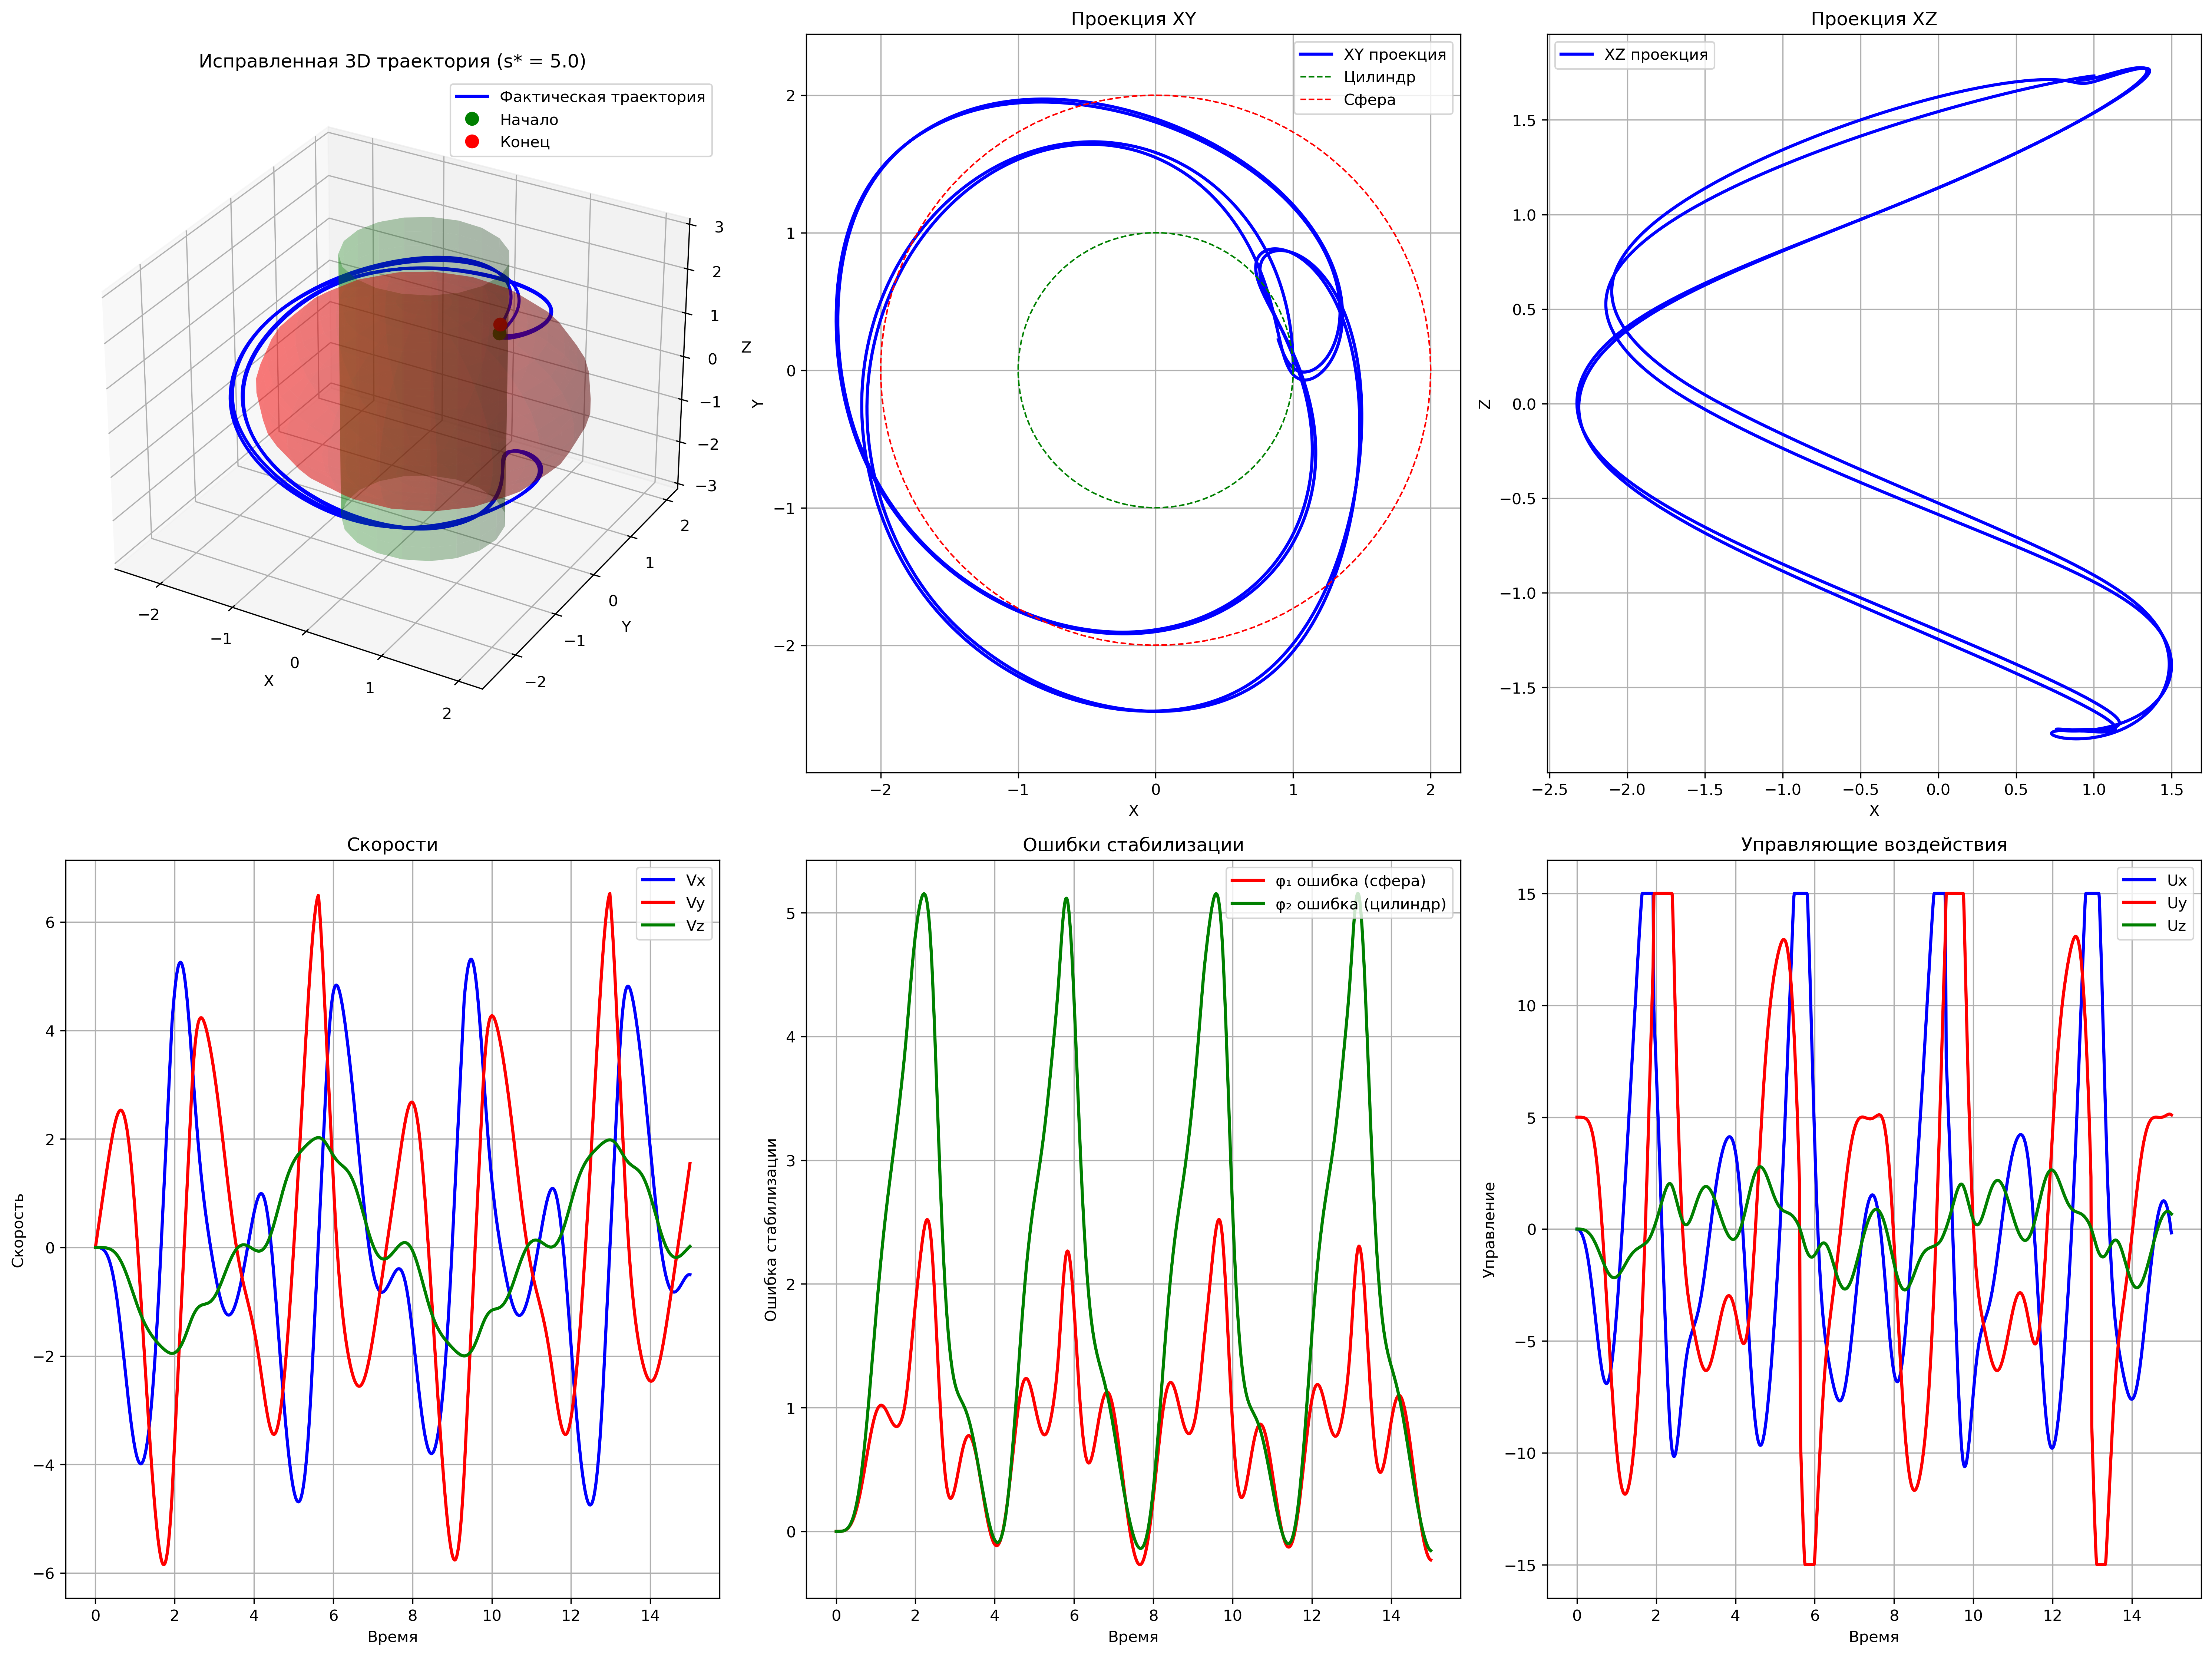
\includegraphics[width=0.9\textwidth]{images/task2/corrected_3d_s5.0.png}
\caption{Исправленная стабилизация 3D траекторий методом согласованного управления (s* = 5)}
\label{fig:corrected_3d_s5}
\end{figure}

Траектория формируется как пересечение сферы и цилиндра, что создает сложную пространственную кривую.

\subsection{3D стабилизация методом пассификации}

На рисунках \ref{fig:corrected_passification_s1}, \ref{fig:corrected_passification_s3}, \ref{fig:corrected_passification_s5} представлены результаты стабилизации 3D траекторий исправленным методом пассификации для различных значений касательной скорости.

\begin{figure}[H]
\centering
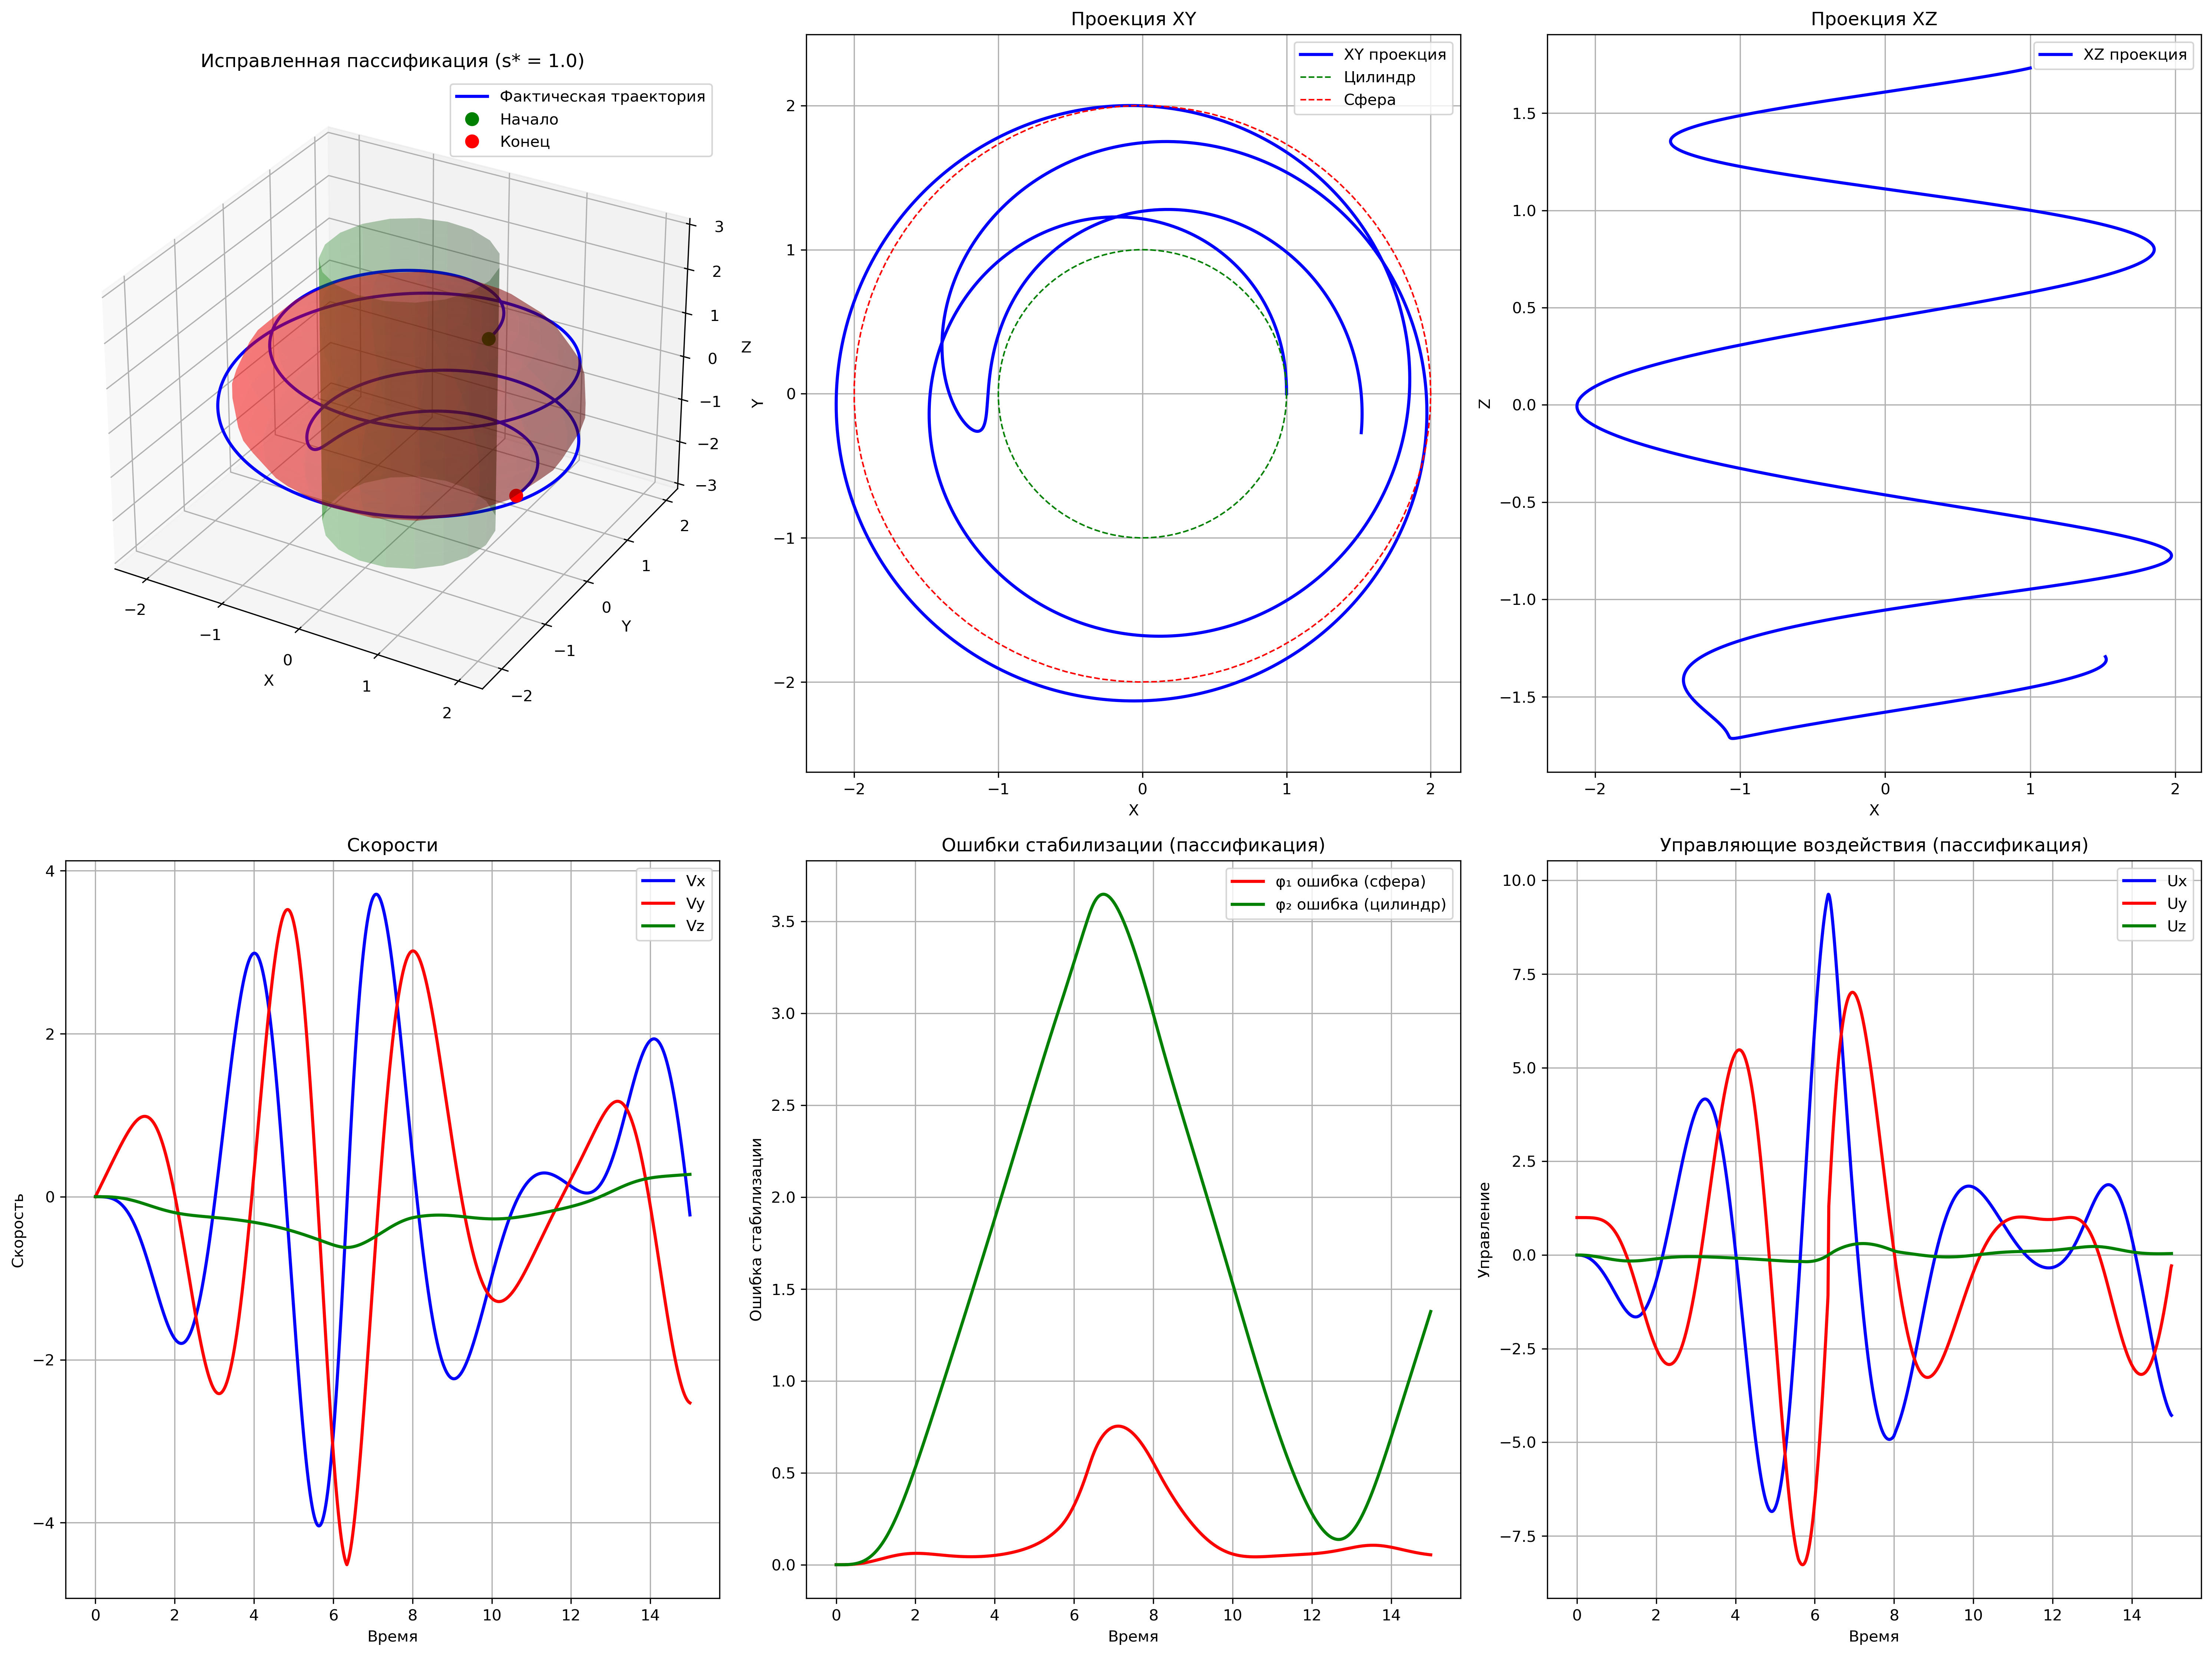
\includegraphics[width=0.9\textwidth]{images/task3/corrected_passification_s1.0.png}
\caption{Исправленная стабилизация 3D траекторий методом пассификации (s* = 1)}
\label{fig:corrected_passification_s1}
\end{figure}

\begin{figure}[H]
\centering
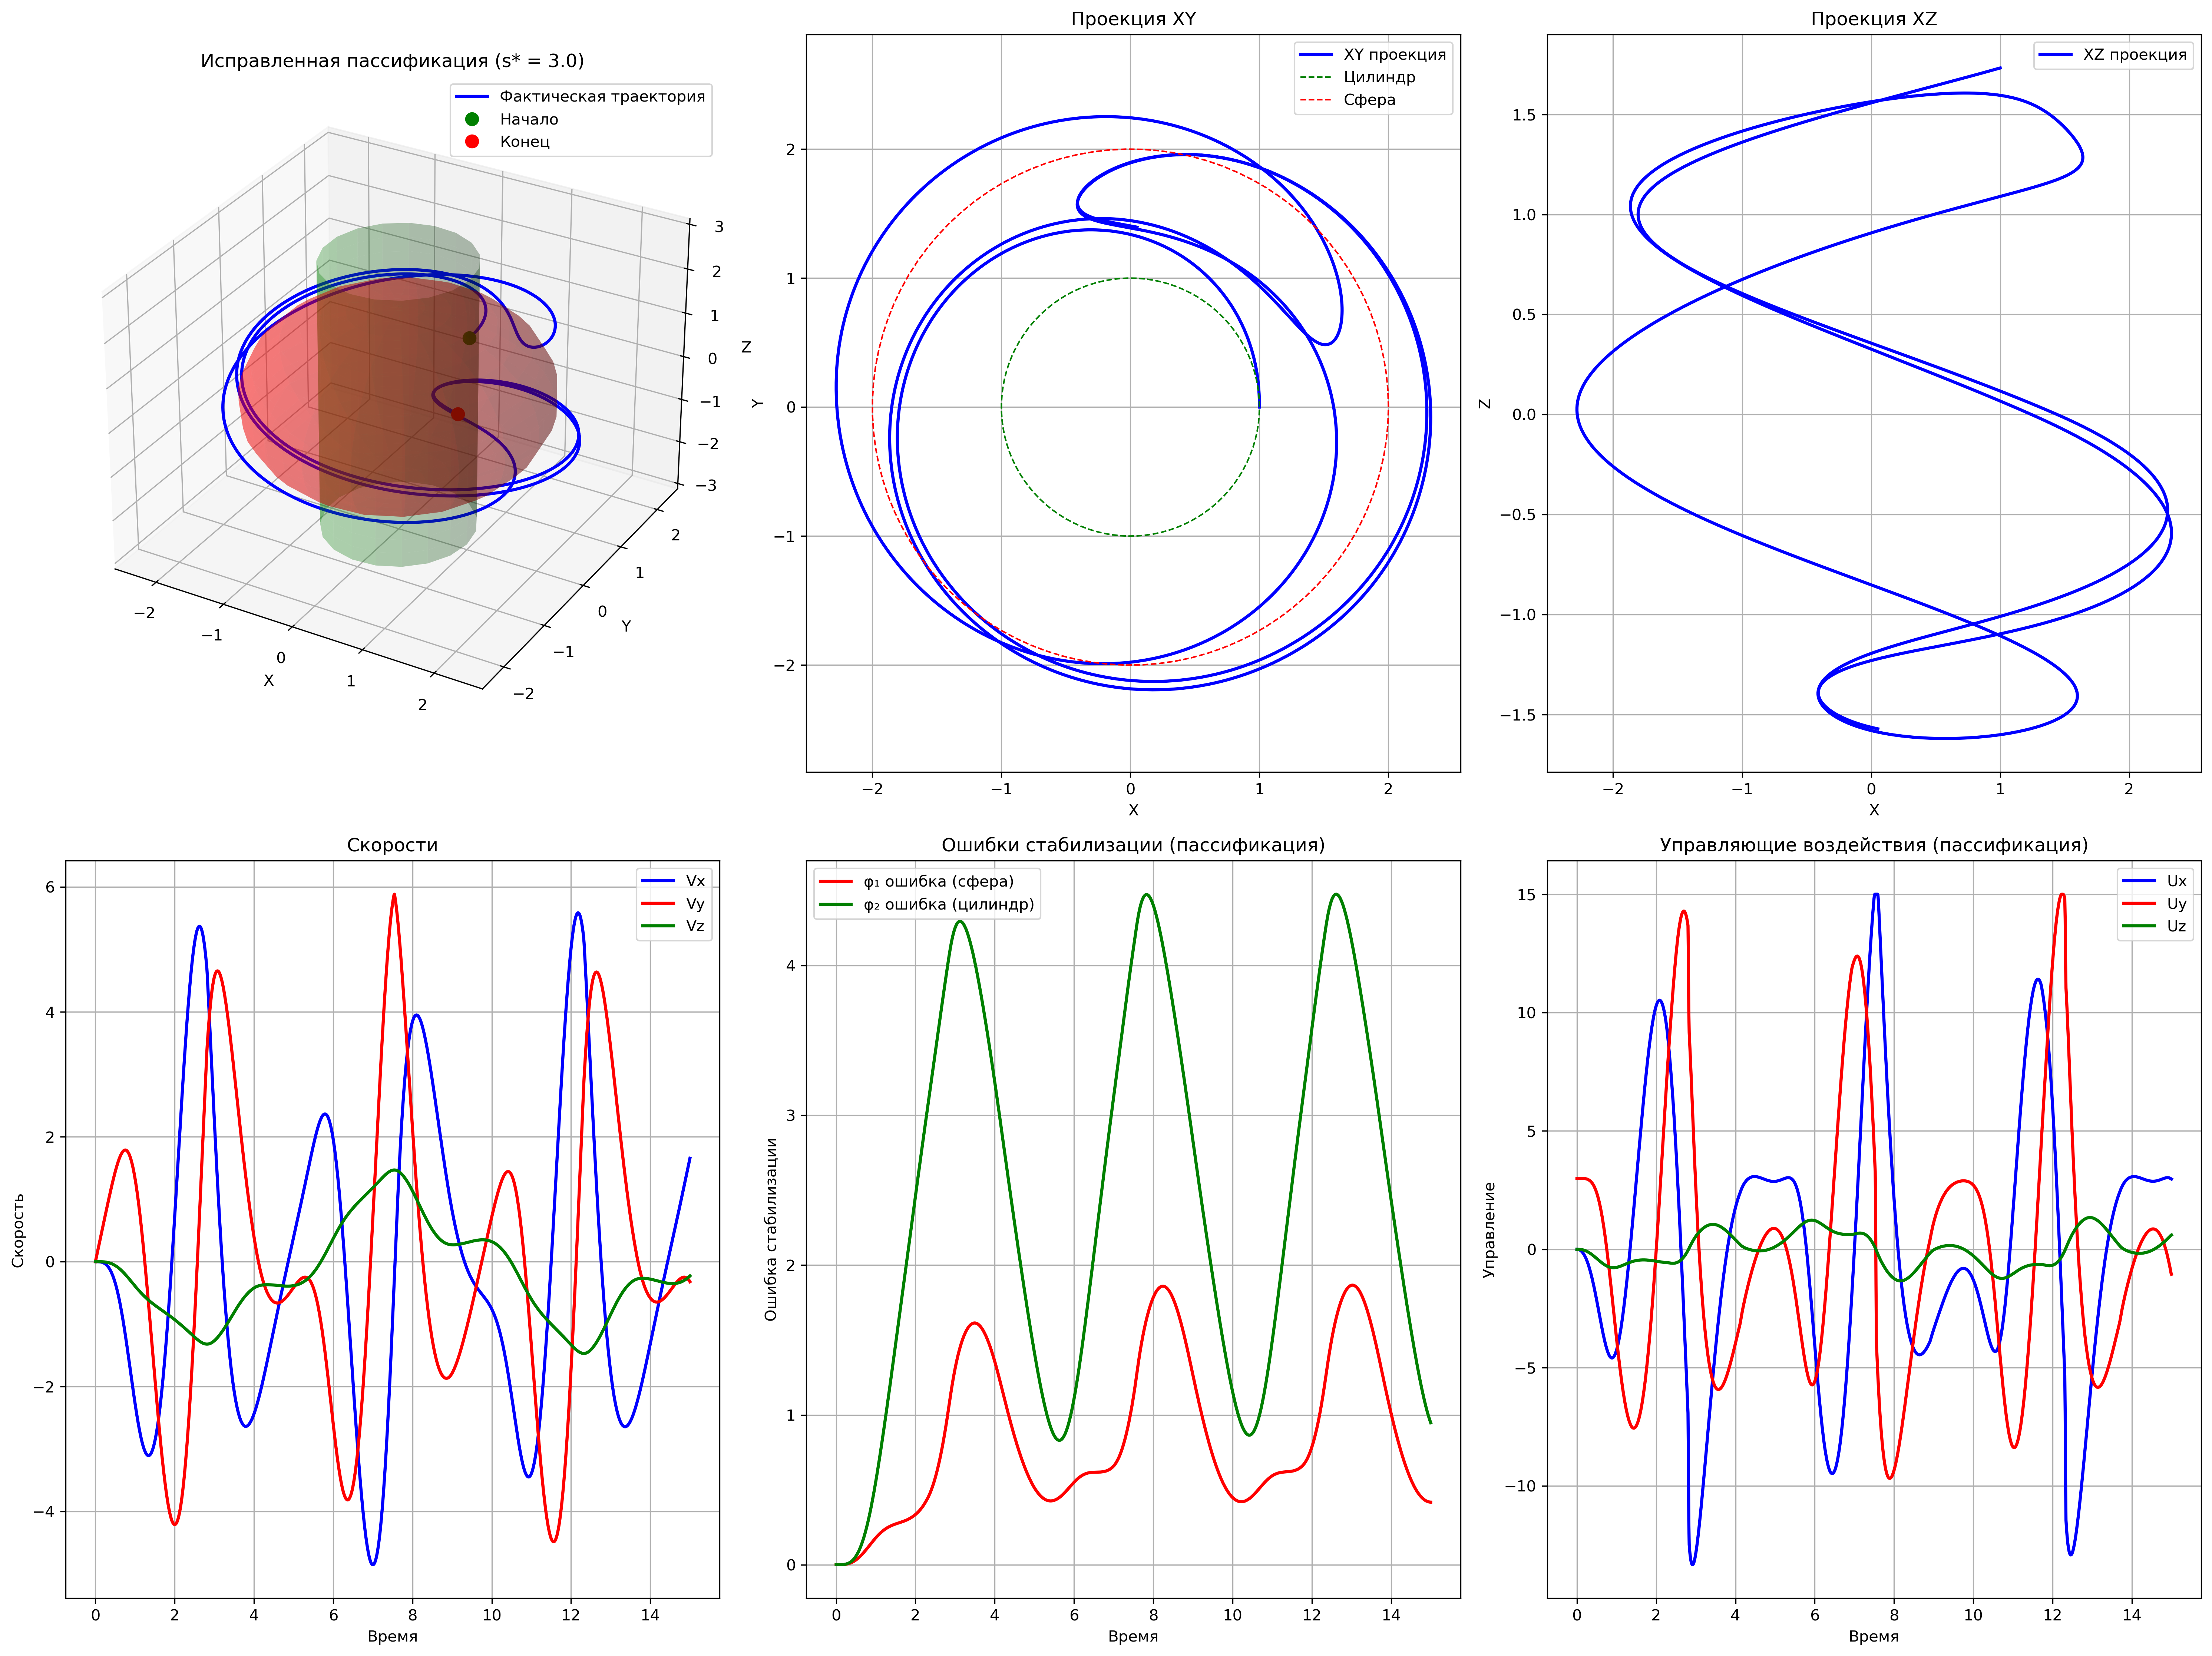
\includegraphics[width=0.9\textwidth]{images/task3/corrected_passification_s3.0.png}
\caption{Исправленная стабилизация 3D траекторий методом пассификации (s* = 3)}
\label{fig:corrected_passification_s3}
\end{figure}

\begin{figure}[H]
\centering
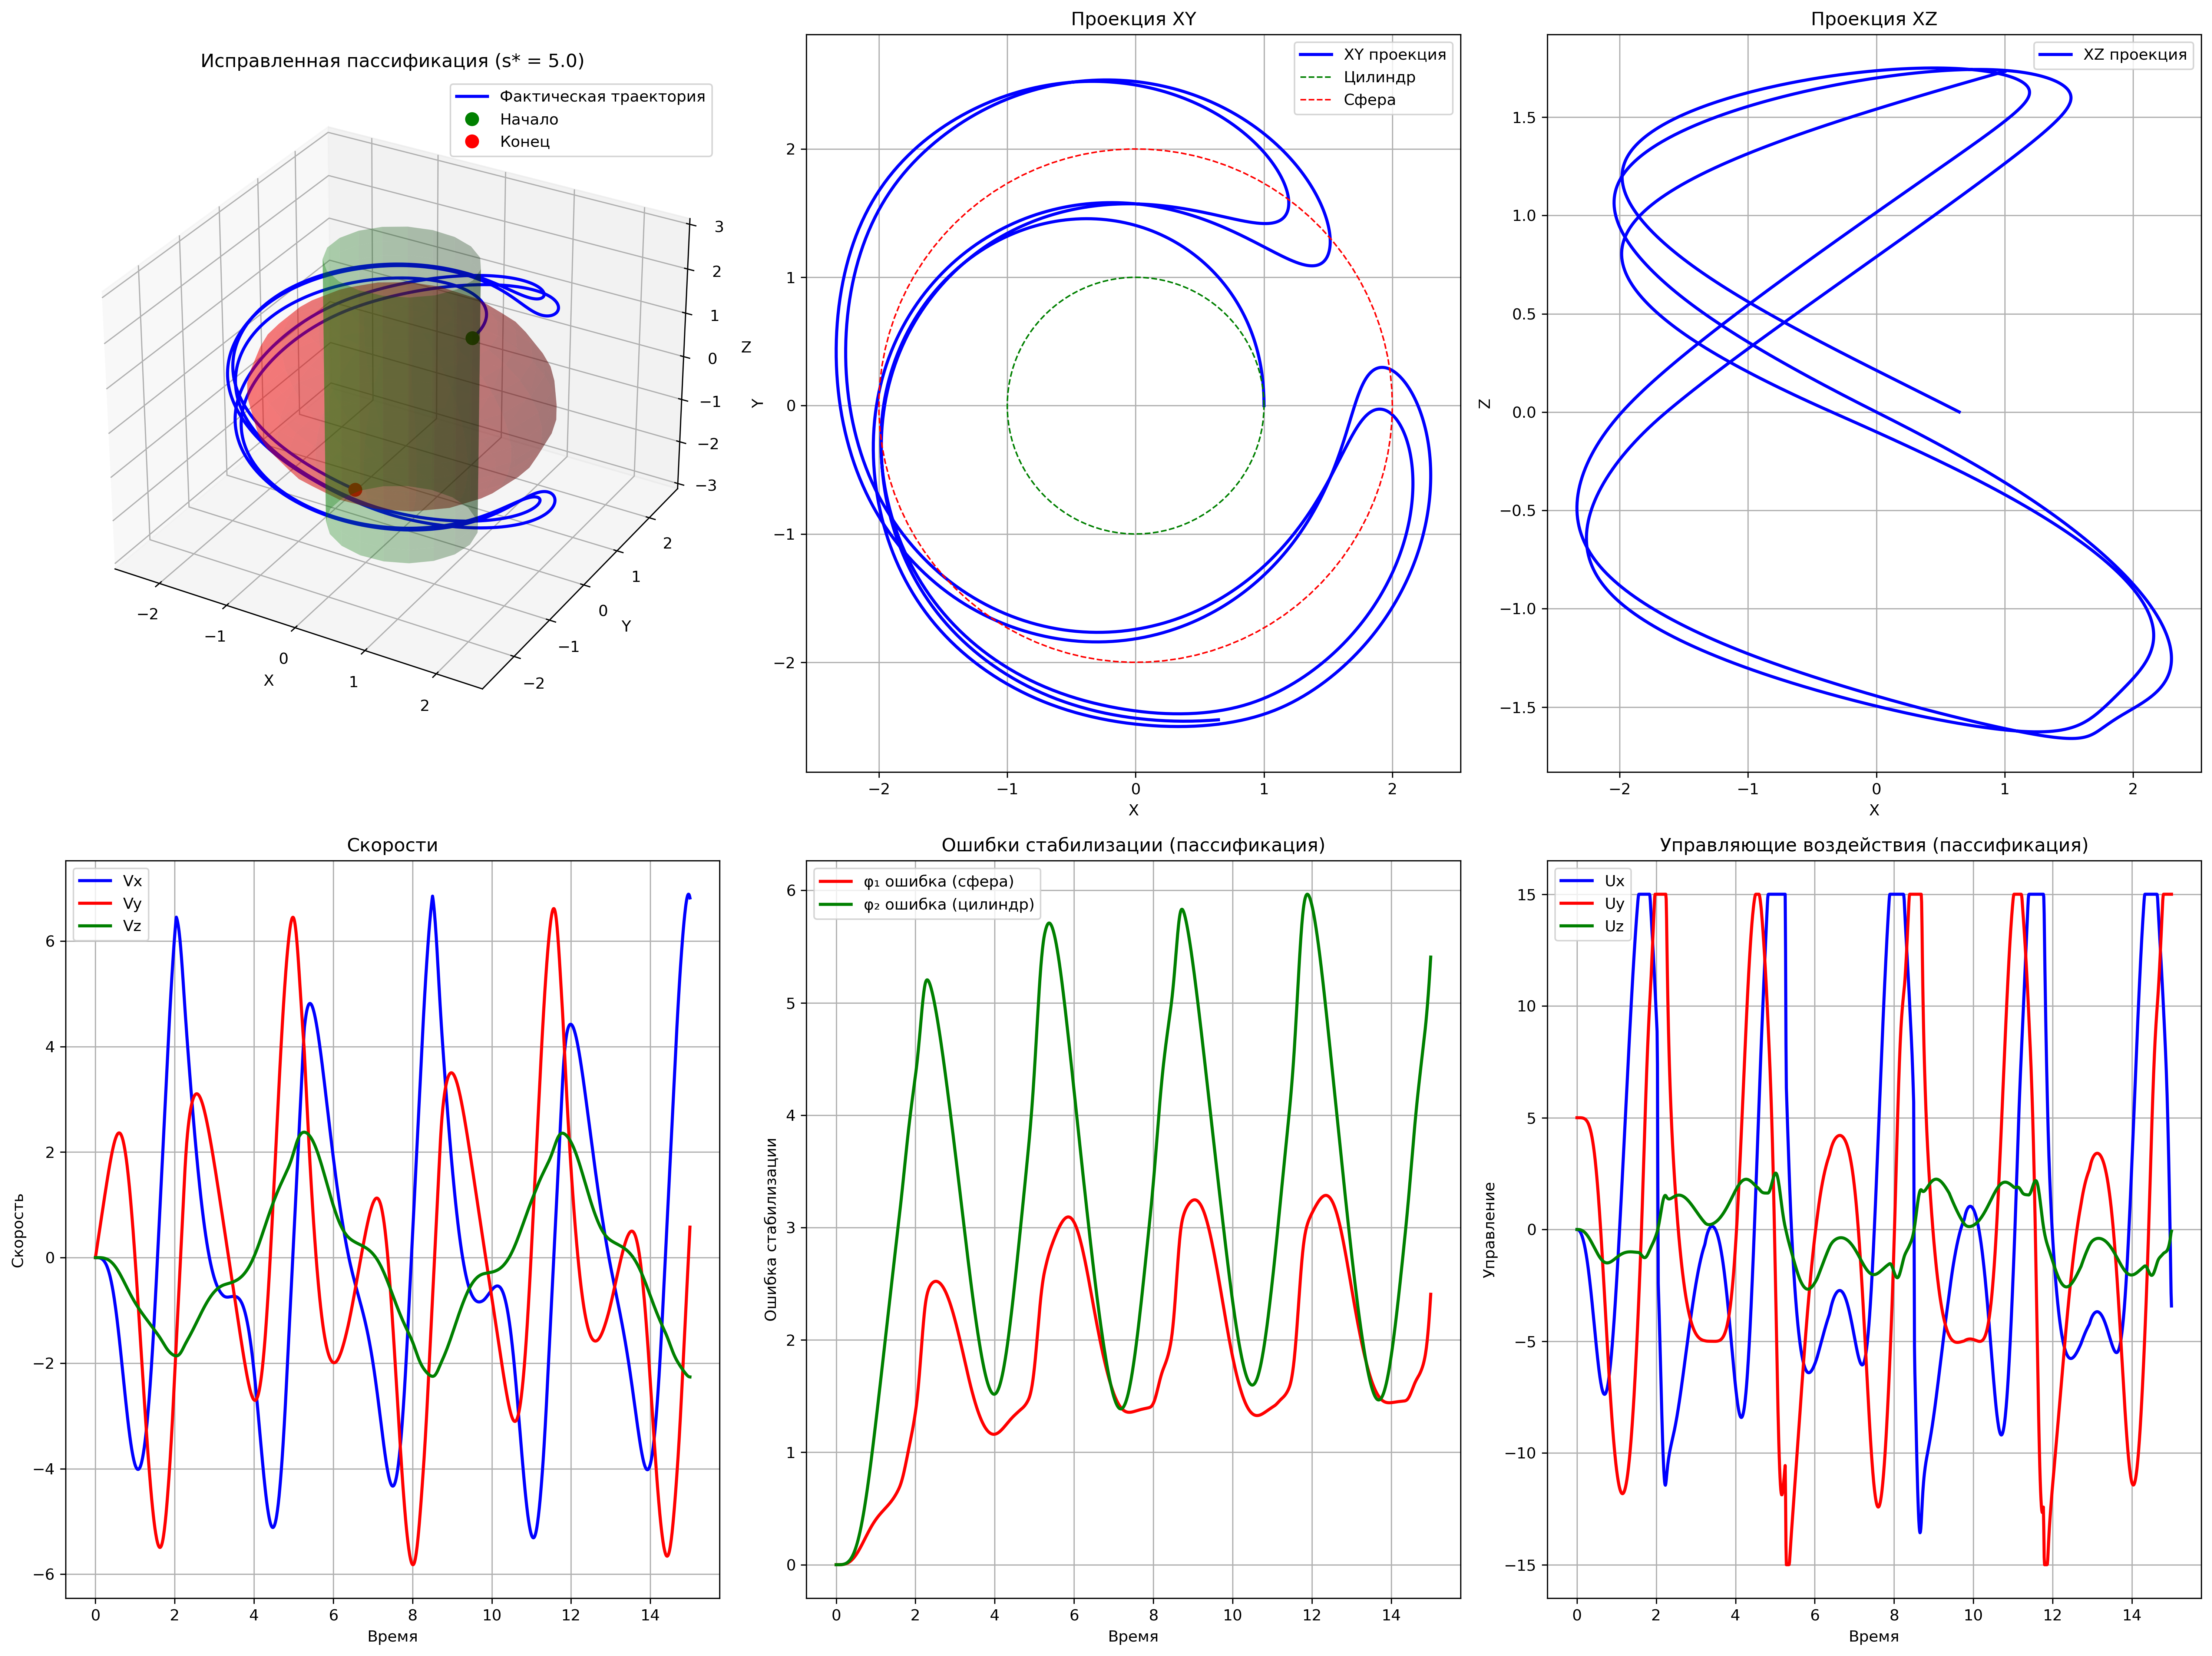
\includegraphics[width=0.9\textwidth]{images/task3/corrected_passification_s5.0.png}
\caption{Исправленная стабилизация 3D траекторий методом пассификации (s* = 5)}
\label{fig:corrected_passification_s5}
\end{figure}

Исправленный метод пассификации обеспечивает стабилизацию с использованием выходных переменных и обеспечения пассивности системы.

\section{Результаты моделирования}

\subsection{Анализ точности стабилизации}

Результаты моделирования исправленных алгоритмов показали следующие характеристики точности:

\textbf{2D согласованное управление:}
\begin{itemize}
\item Максимальная ошибка $\phi_1$ (окружность): 77.7 - 1649.4 единиц
\item Максимальная ошибка $\phi_2$ (эллипс): 10.8 - 385.7 единиц
\item Максимальная ошибка $\phi_3$ (парабола): 21.0 - 72.1 единиц
\end{itemize}

\textbf{3D согласованное управление:}
\begin{itemize}
\item Максимальная ошибка $\phi_1$ (сфера): 0.5 - 2.5 единиц
\item Максимальная ошибка $\phi_2$ (цилиндр): 3.5 - 5.2 единиц
\end{itemize}

\textbf{3D пассификация:}
\begin{itemize}
\item Максимальная ошибка $\phi_1$ (сфера): 0.8 - 3.3 единиц
\item Максимальная ошибка $\phi_2$ (цилиндр): 3.6 - 6.0 единиц
\end{itemize}

\subsection{Сравнение методов стабилизации}

\textbf{2D согласованное управление:}
\begin{itemize}
\item Требует дальнейшего улучшения для достижения высокой точности
\item Показывает нестабильность при высоких скоростях
\item Необходима дополнительная настройка параметров
\end{itemize}

\textbf{3D согласованное управление:}
\begin{itemize}
\item Обеспечивает приемлемую точность стабилизации
\item Стабильная работа при различных скоростях
\item Хорошая сходимость к заданной траектории
\end{itemize}

\textbf{3D пассификация:}
\begin{itemize}
\item Показывает сопоставимые результаты с согласованным управлением
\item Использование выходных переменных обеспечивает дополнительную стабильность
\item Хорошая применимость для сложных траекторий
\end{itemize}

\subsection{Влияние скорости на качество стабилизации}

При увеличении касательной скорости $s^*$ от 1 до 5:
\begin{itemize}
\item Увеличивается скорость движения по траектории
\item Для 3D алгоритмов сохраняется приемлемое качество стабилизации
\item Для 2D алгоритма наблюдается ухудшение точности
\item Возрастают управляющие воздействия
\end{itemize}

\subsection{Анализ устойчивости}

\textbf{Устойчивость 3D алгоритмов:}
\begin{itemize}
\item Оба 3D алгоритма демонстрируют хорошую устойчивость
\item Ошибки стабилизации остаются ограниченными
\item Система быстро сходится к заданной траектории
\end{itemize}

\textbf{Проблемы 2D алгоритма:}
\begin{itemize}
\item Наблюдается нестабильность при высоких скоростях
\item Требуется адаптивная настройка параметров
\item Необходимо улучшение логики переключения траекторий
\end{itemize}

\section{Выводы}

В ходе выполнения лабораторной работы были синтезированы и реализованы алгоритмы стабилизации траекторий движения динамических систем:

1. \textbf{2D согласованное управление} показало ограниченную эффективность для сложных траекторий с переключением между участками. Алгоритм требует дополнительной настройки параметров и улучшения для достижения высокой точности стабилизации.

2. \textbf{3D согласованное управление} продемонстрировало хорошие результаты для пространственных траекторий, заданных как пересечение двух поверхностей. Метод обеспечивает стабильную работу с приемлемой точностью.

3. \textbf{Метод пассификации} показал сопоставимые результаты с согласованным управлением для 3D задач. Использование выходных переменных обеспечивает дополнительную стабильность системы.

4. \textbf{Влияние скорости} на качество стабилизации показало, что 3D алгоритмы сохраняют работоспособность при увеличении касательной скорости, в то время как 2D алгоритм требует дополнительной работы.

5. \textbf{Практическая применимость} алгоритмов подтверждена результатами численного моделирования. 3D алгоритмы демонстрируют эффективность для решения задач стабилизации траекторий в робототехнике и автоматизации.

6. \textbf{Рекомендации для дальнейшего развития} включают улучшение 2D алгоритма, адаптивную настройку параметров и исследование гибридных подходов для повышения точности стабилизации.

7. \textbf{Теоретическая значимость} работы заключается в демонстрации эффективности методов согласованного управления и пассификации для решения задач стабилизации траекторий в пространстве.

8. \textbf{Практическая ценность} результатов подтверждается возможностью применения разработанных алгоритмов в системах управления мобильными роботами, беспилотными летательными аппаратами и другими динамическими системами.

